% !TEX root = ../../Dissertation.tex

\begin{refsection}




\chapter[Bimetallic C\lowercase{r}-M\lowercase{n} Oxide Clusters]{Geometric Structures, Structural Evolution, and Magnetic Properties of Hybrid Chromium Manganese Oxide Clusters} \label{CrMnO}


\definecolor{shadecolor}{gray}{0.85}
\begin{shaded}
\textbf{This chapter is based on the manuscript:}\\
Pham, L. N.; van Dijk, C. N.; Kirilyuk, A.; Nguyen, M. T.; Janssens, E. et al. Bimetallic Oxide Clusters \ch{Cr_xMn_yO_z+}: Geometric structures, structural evolution, and magnetic properties \textit{Manuscript in preparation}. \textcolor{blue}{The \href{https://github.com/phamlenhan/PhDDissertation/blob/master/Chapter-8SI-Nhan-thesis-CrMnO.pdf}{Supporting Information} is available online}.

\emph{My contribution to this work was theoretical calculations, data analysis, discussion, and writing of the first draft.}
\newpage
\end{shaded}


\section{Introduction}

Chromium and manganese are two first row transition metal elements with atomic elemental configurations that have five singly occupied 3\textit{d} orbitals ([Ar]3d$^5$4s$^1$ and [Ar]3d$^5$4s$^2$). The electronic ground states of the neutral \ch{Cr2} and \ch{Mn2} dimers are singlets due to antiferromagnetic coupling between the local spin magnetic moments on the atoms. \cite{Baumann83, Bier88, Vanzee81, Yamamoto06, Bondybey83, Cr2+} However, the ground states of the cationic dimers possess high-spin magnetic moments (11$\mu_B$) as a result of ferromagnetic coupling. \cite{Cr2+, Mn2+, Vanzee88} Considering the bimetallic CrMn dimer, the local magnetic moments are ferrimagnetically coupled, leading to a small net magnetic moment of 3 $\mu_B$. \cite{Mn2+, Desmarais00} In larger clusters, the magnetic behaviors of chromium and manganese gradually diverge. \ch{Cr3} was found to have a quartet ground state as a result of ferrimagnetic coupling, \cite{Nhan18} while in \ch{Mn3} ferrimagnetic and ferromagnetic states were found to be energetically competitive. \cite{Gutsev2006, Bobadova2003, Pederson98, Longo2005} The energetic competition between ferrimagnetism and ferromagnetism as the ground state of \ch{Mn4} is less clear. \cite{Pederson98, Bobadova2003} An energetic competition between two ferrimagnetic states (S = 1 vs. S = 6) was predicted for \ch{Cr4}. \cite{Cr4} In bulk materials, chromium is antiferromagnetic at room temperature,\cite{Fawcett1988} while the stable $\alpha$ phase of manganese is paramagnetic. \cite{Hobbs03} Above 311 K, bulk chromium is paramagnetic as well. \cite{Fawcett1988}  




An effective way to modify and control magnetic properties of transition metal clusters is to introduce a different element, such as oxygen, into clusters. Indeed, total spin magnetic moments of small chromium oxide clusters (\ch{Cr2O_n}, n = 1 -- 3 \cite{Tono2003, Tono2003B, paulCr2On} and \ch{Cr3O_n+}, n = 0 -- 5 \cite{Nhan18}) were found to be strongly dependent on the number of oxygen atoms. Superexchange-type, 3\textit{d}-3\textit{d} bonding-like interactions, and 3\textit{d}-2\textit{p} delocalization were found to dominate the magnetic evolution of these clusters. As for manganese oxide clusters, total magnetic moments of \ch{Mn2O^{-/0}} and \ch{Mn2O2+} also seem to vary with the addition of oxygen atoms. \cite{Khanna04, Marks18} Experiments indicated that ferromagnetic and antiferromagnetic configurations coexist for the case of \ch{Mn2O^{-/0}}. \cite{Khanna04} Computations predicted an energetic competition between 2-tet and 10-tet states in \ch{Mn2O2+}. \cite{Marks18} For clusters with a larger number of oxygen atoms (n = 3 -- 7), the total magnetic moments of \ch{Mn2O_n^{-/0/+}} do not significantly change. \cite{Gutsev18} A systematic study has not been done for the series of \ch{Mn3O_n+}, but for \ch{Mn3O3+} a spin quintet state was theoretically predicted. \cite{Marks18} In this case, the spin state of \ch{Mn3O3+} is much lower than that of \ch{Cr3O3+} (12-tet). \cite{Nhan18} In large manganese oxides clusters, addition of oxygen atoms is believed to cause alteration of total magnetic moments. \cite{Williams12} 



As can be seen from the abovementioned studies, two popular types of experimental signals possibly obtained from synthesized clusters are photoelectron spectra and infrared photodissociation spectra. The latter gives direct information about the geometrical structures of studied clusters. Different magnetic configurations typically have (slightly) different geometric configurations, and as a result, their IR spectra are different. Surprisingly, for specific cases, the overall geometrical structures are similar, but a different magnetic configuration can lead to a different IR spectrum. The neutral \ch{Fe4O4} cluster is a good example of a cluster for which a single geometric motif can expose three magnetic moments of 0, 10 and 20 $\mu_B$. \cite{fe4o6Ding, fe4o6Kirilyuk, fe4o6Logemann, fe4o6Erlebach} Or in our very recent work, a small change in geometry of \ch{Co_nCr+} (n = 3, 4) clusters can produce different total magnetic moments due to energetic degeneracy of several spin states. \cite{Meyei18} Therefore, geometries of clusters need to be accurately determined. In doing so, \acrshort{irmpd} spectra are used as reference for finding the best match with simulated harmonic vibrational spectra of different structural isomers, obtained from quantum chemical calculations. \cite{fe4o6Logemann, Janssens01, Sant2008, Mathias03, Asmis07, Nhan18, Dijk14}  For specific cases, \acrshort{irmpd} can be an appropriate tool used to distinguish spin configurations of clusters with a same or similar geometric motif, \cite{Nhan18} which sheds light on apparent relation between magnetic properties and \acrshort{irmpd} spectra.   



While various studies on chromium and manganese oxide clusters have been performed, the corresponding bimetallic oxide clusters are unexplored. A few works were conducted to investigate magnetic properties and crystal structures of bulk chromium-manganese oxides such as \ch{CrMnO3} and \ch{CrMnO4}. \cite{Nalbandyan13, Chamberland77} In the current work, we synthesized multiple bimetallic oxide clusters and characterized them spectroscopically with the \acrshort{irmpd} technique. In combination with quantum chemical methods, geometrical and electronic structures of the synthesized clusters are unveiled. On the basis of obtained geometries and electronic features, magnetic interactions between metallic sites, and size and composition dependent magnetic evolution of \ch{Cr_xMn_yO_z+} (x + y = 2 -- 4, z = 4 --9) are disclosed.  






%\section{Experimental method}

 

%The cluster cations are produced by ablating the metal (Chris - specify target alloy? which composition 505/50?) with the second harmonic output 532 nm, 10 mJ (ok?) of a pulsed Nd-YAG laser and quenching the plasma with a short pulse of a gas mixture containing 0.5\% ($ok?$) oxygen in helium. After expansion into vacuum the cluster distribution is analyzed using a reflectron time-of-flight mass spectrometer. The cluster beam is overlapped with a counter-propagating  infrared laser beam, delivered by the free electron laser for infrared experiments FELIX, providing intense $micros$ long pulses of tunable IR radiation in the 40 -- 2500 cm$^{-1}$ range (see refxxx). The resonant absorption of photons by a specific cluster is detected by monitoring the dissociation of weakly bound cluster complexes. In particular, here we monitor the dissociation of oxygen rich cationic \ch{CrMnO_m+} clusters is monitored through the evaporation of \ch{O2} molecules. This is observed through a simultaneous decrease of the mother \ch{Cr_nMnO_m+} signal and an increase of the \ch{Cr_nMnO_{m-2}+} daughter signal in the mass spectrometer. Infrared multiple photon dissociation (\acrshort{irmpd} spectra) are constructed by recording the ion intensities of the clusters, both parents and products, as a function of the FELIX frequency. The spectra shown are of the difference between the loss in the educt and the increase in the product in the mass spectra as a function of FELIX wavelength. Note that all experiments are performed on nascent (positive) ions, that is clusters that already have a charge when leaving the cluster source. The advantage here is that no post-ionisation is required, a process that can inadvertently induce the dissociation of the cluster-messenger complex. In general, bands above 1000 cm$^{-1}$ correspond to O=O stretch modes of the dioxygen messenger, and give clues as to the nature of the bonding between the messenger and the cluster. Bands below 1000 cm$^{-1}$ however typically correspond to O=O symmetric and asymmetric stretching within the cluster itself, and can thus provide a `fingerprint' of the structure of the cluster (especially when delocalised modes are probed).


\section{Methodology}

All the clusters in this chapter were synthesized by employing the same technique that was described in Chapter \ref{CrxOy}. The significant difference here is that the messenger species used is \ch{O2}. After the synthesis and \acrshort{irmpd} measurement, quantum chemical computations were conducted. The computational procedure that was followed consists of three main steps. First, for each composition, a large numbers of initial isomers was generated by use of the CALYPSO tool, \cite{CALYPSO} and geometrically optimized at the fast B3LYP \cite{lyp,b3lyp2,b3} and BP86 \cite{b3lyp2,p86} levels in combination with the small 3-21G basis set. \cite{3-21G-2nd, 3-21G-tran} For each size a maximum of 50 low-energy structures were screened and pushed to the next geometrical optimization step with a larger triple-$\zeta$ basis set def2-TZVP. \cite{def2} In the second step, three density functionals (TPSS, \cite{tpss} BP86, \cite{b3lyp2,p86} and B3P86 \cite{b3,p86}) were employed to reoptimize the geometries without any symmetry constraint. For clusters without experimental data, only the TPSS functional was employed. For the purpose of comparison, additional oxide clusters of chromium were also geometrically optimized making use of the TPSS functional.\cite{tpss} To ensure that all low-lying isomers are minima on the potential energy hypersurface, harmonic vibrational frequencies were calculated analytically. The TPSS, BP86, and B3P86 functionals were used because these functionals were found to give good results on geometries and vibrational frequencies of chromium oxide clusters. \cite{Nhan18} Beside the use of the CALYPSO tool to generate initial structures, several isomers were also built on the basis of smaller cluster sizes. Especially, for clusters with the same number of metallic atoms but different metallic ratios, permutations were applied to the metal atoms to draw other low-lying isomers. This process increases our capability to correctly identify low-energy isomers. The third and last step of the computational approach dealt with simulating the effect of molecular oxygen on the vibration spectra, since the oxygen molecules are used in the experiment as messenger for the adsorption of the infrared red. Due to the energy used in the experiment to break two oxygen atoms attached on the clusters is in the range of 15--30 meV, we believe that the \ch{O2} group weakly binds to the cluster. Therefore, the effect of oxygen gas messenger was, then, treated by considering the clusters \ch{Cr_xMn_yO_z+} with attached \ch{O2} in simulation of IR spectra. Since all simulated frequencies of terminal metal-O vibrations are overestimated in comparison to the experimental ones, this mode of vibrations was scaled with a factor of 0.93. This scaling value was chosen because it gave better agreement with the experiment among several tested values. All remaining modes are kept unchanged. Quantum chemical calculations were done with the Gaussian 09 program, \cite{g09} and dispersion corrections were taken into account using the DFT-D3 parameters \cite{GD3} for the supported functionals (TPSS and BP86).   




\section{Results and discussion}

\subsection{Structural assignments}

\subsubsection{\ch{CrMnO4+}}
	
In this work, \ch{CrMnO4+} is the smallest bimetallic cluster synthesized and spectroscopically characterized with well-resolved \acrshort{irmpd} signals. Its \acrshort{irmpd} spectrum is given in Figure \ref{fig:CrMnOx}. A quintet $^5$A state was found to be the most stable for \ch{CrMnO4+}. The experimental \acrshort{irmpd} spectrum of \ch{CrMnO4+}, measured by depletion of \ch{CrMnO4^{+}O2} (Figure \ref{fig:CrMnOx}), has two clear bands at 670 and 1010 cm$^{-1}$. The simulated spectrum of the obtained ground state structure reproduces the band at 670 cm$^{-1}$, while the higher energy mode is blueshifted by 70 cm$^{-1}$ in the simulation (without consideration of scaling). The simulated spectrum of \ch{CrMnO4^{+}O2} in Figure \ref{fig:CrMnOx}c has an additional band at around $\sim$1200 cm$^{-1}$ corresponding to the \ch{O=O} stretching mode, which is in good agreement with the experimental one even though the intensity of this band is much higher than that of the experiment. From all above features, we believe that the \ch{CrMnO4^{+}} isomer wih attached \ch{O2} (\ch{CrMnO4^{+}O2}) was measured in the experiment. Note that the other two isomers of \ch{CrMnO4+} shown in Figure \href{https://github.com/phamlenhan/PhDDissertation/blob/master/Chapter-8SI-Nhan-thesis-CrMnO.pdf}{\textcolor{blue}{S2}}\commenttext{\ref{SI:figs:CrMnO4}} of the \href{https://github.com/phamlenhan/PhDDissertation/blob/master/Chapter-8SI-Nhan-thesis-CrMnO.pdf}{\textcolor{blue}{Supporting Information (SI)}} have a significantly higher relative energy and cannot reproduce the experimental \acrshort{irmpd} bands of < 1100 cm$^{-1}$ (see Figure \href{https://github.com/phamlenhan/PhDDissertation/blob/master/Chapter-8SI-Nhan-thesis-CrMnO.pdf}{\textcolor{blue}{S40}}\commenttext{\ref{SI:figs:CrMnO4-spec-si}}).


\begin{figure}
	\centering
	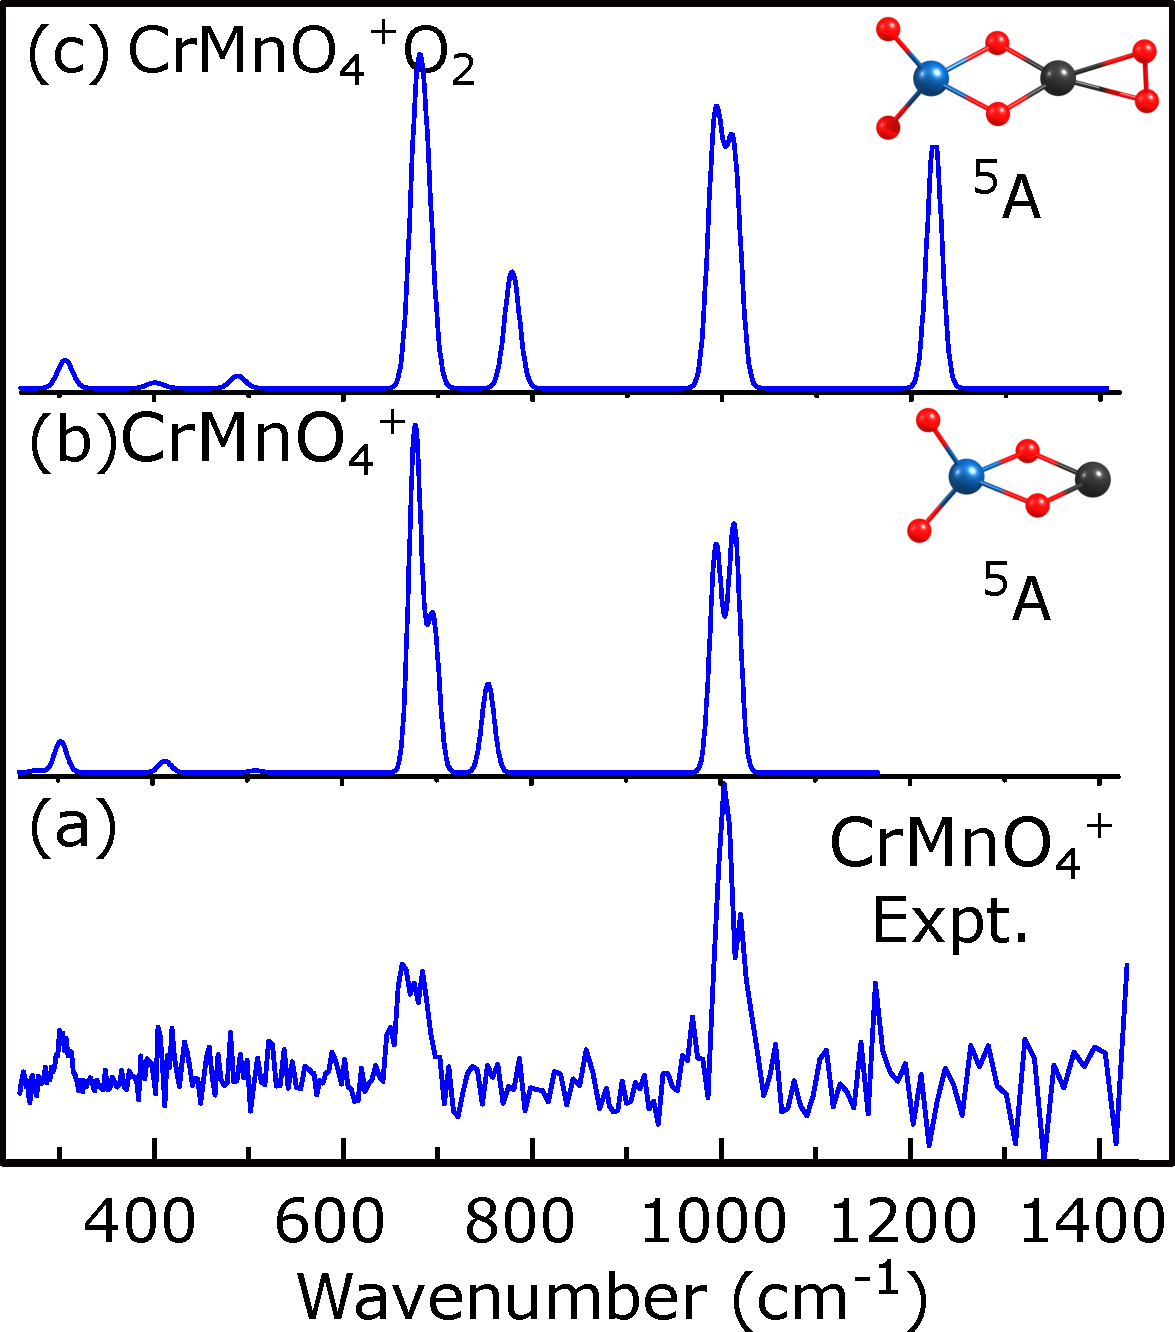
\includegraphics[width=0.4\linewidth]{CrMnO4}
	\caption{Experimental \acrshort{irmpd} and simulated (at the TPSS level) harmonic IR spectra of low-energy isomers of \ch{CrMnO4+}. The geometrical structures of selected low-lying states are given as inset with chromium (manganese) atoms represented by blue (black) balls.}
	\label{fig:CrMnOx}
\end{figure}

%\textcolor{blue}{Discuss the mother and daughter.O2 simulated spectra}


\subsubsection{\ch{Cr_xMn_yO_z+} (x + y = 3, z = 5 - 7)}


Four bimetallic clusters  containing three metal atoms were studied: \ch{CrMn2O5+}, \ch{CrMn2O6+}, \ch{Cr2MnO6+}, and \ch{Cr2MnO7+}. The experimental \acrshort{irmpd} spectra of these clusters are presented in Figures \ref{fig:CrMn2Oz} and \ref{fig:Cr2MnOz}. Except for the spectrum of \ch{Cr2MnO7+}, their spectra reveal the \ch{O=O} stretching mode around 1200 cm$^{-1}$, which is representative for the \ch{O2} group that is used as messenger in the experiment. The vibrational modes around $\sim$1000 cm$^{-1}$ correspond to vibrations of terminal oxygen atoms while the remaining lower-frequency modes are associated with vibrations of the main frames of the clusters. 

\begin{figure}
	\centering
	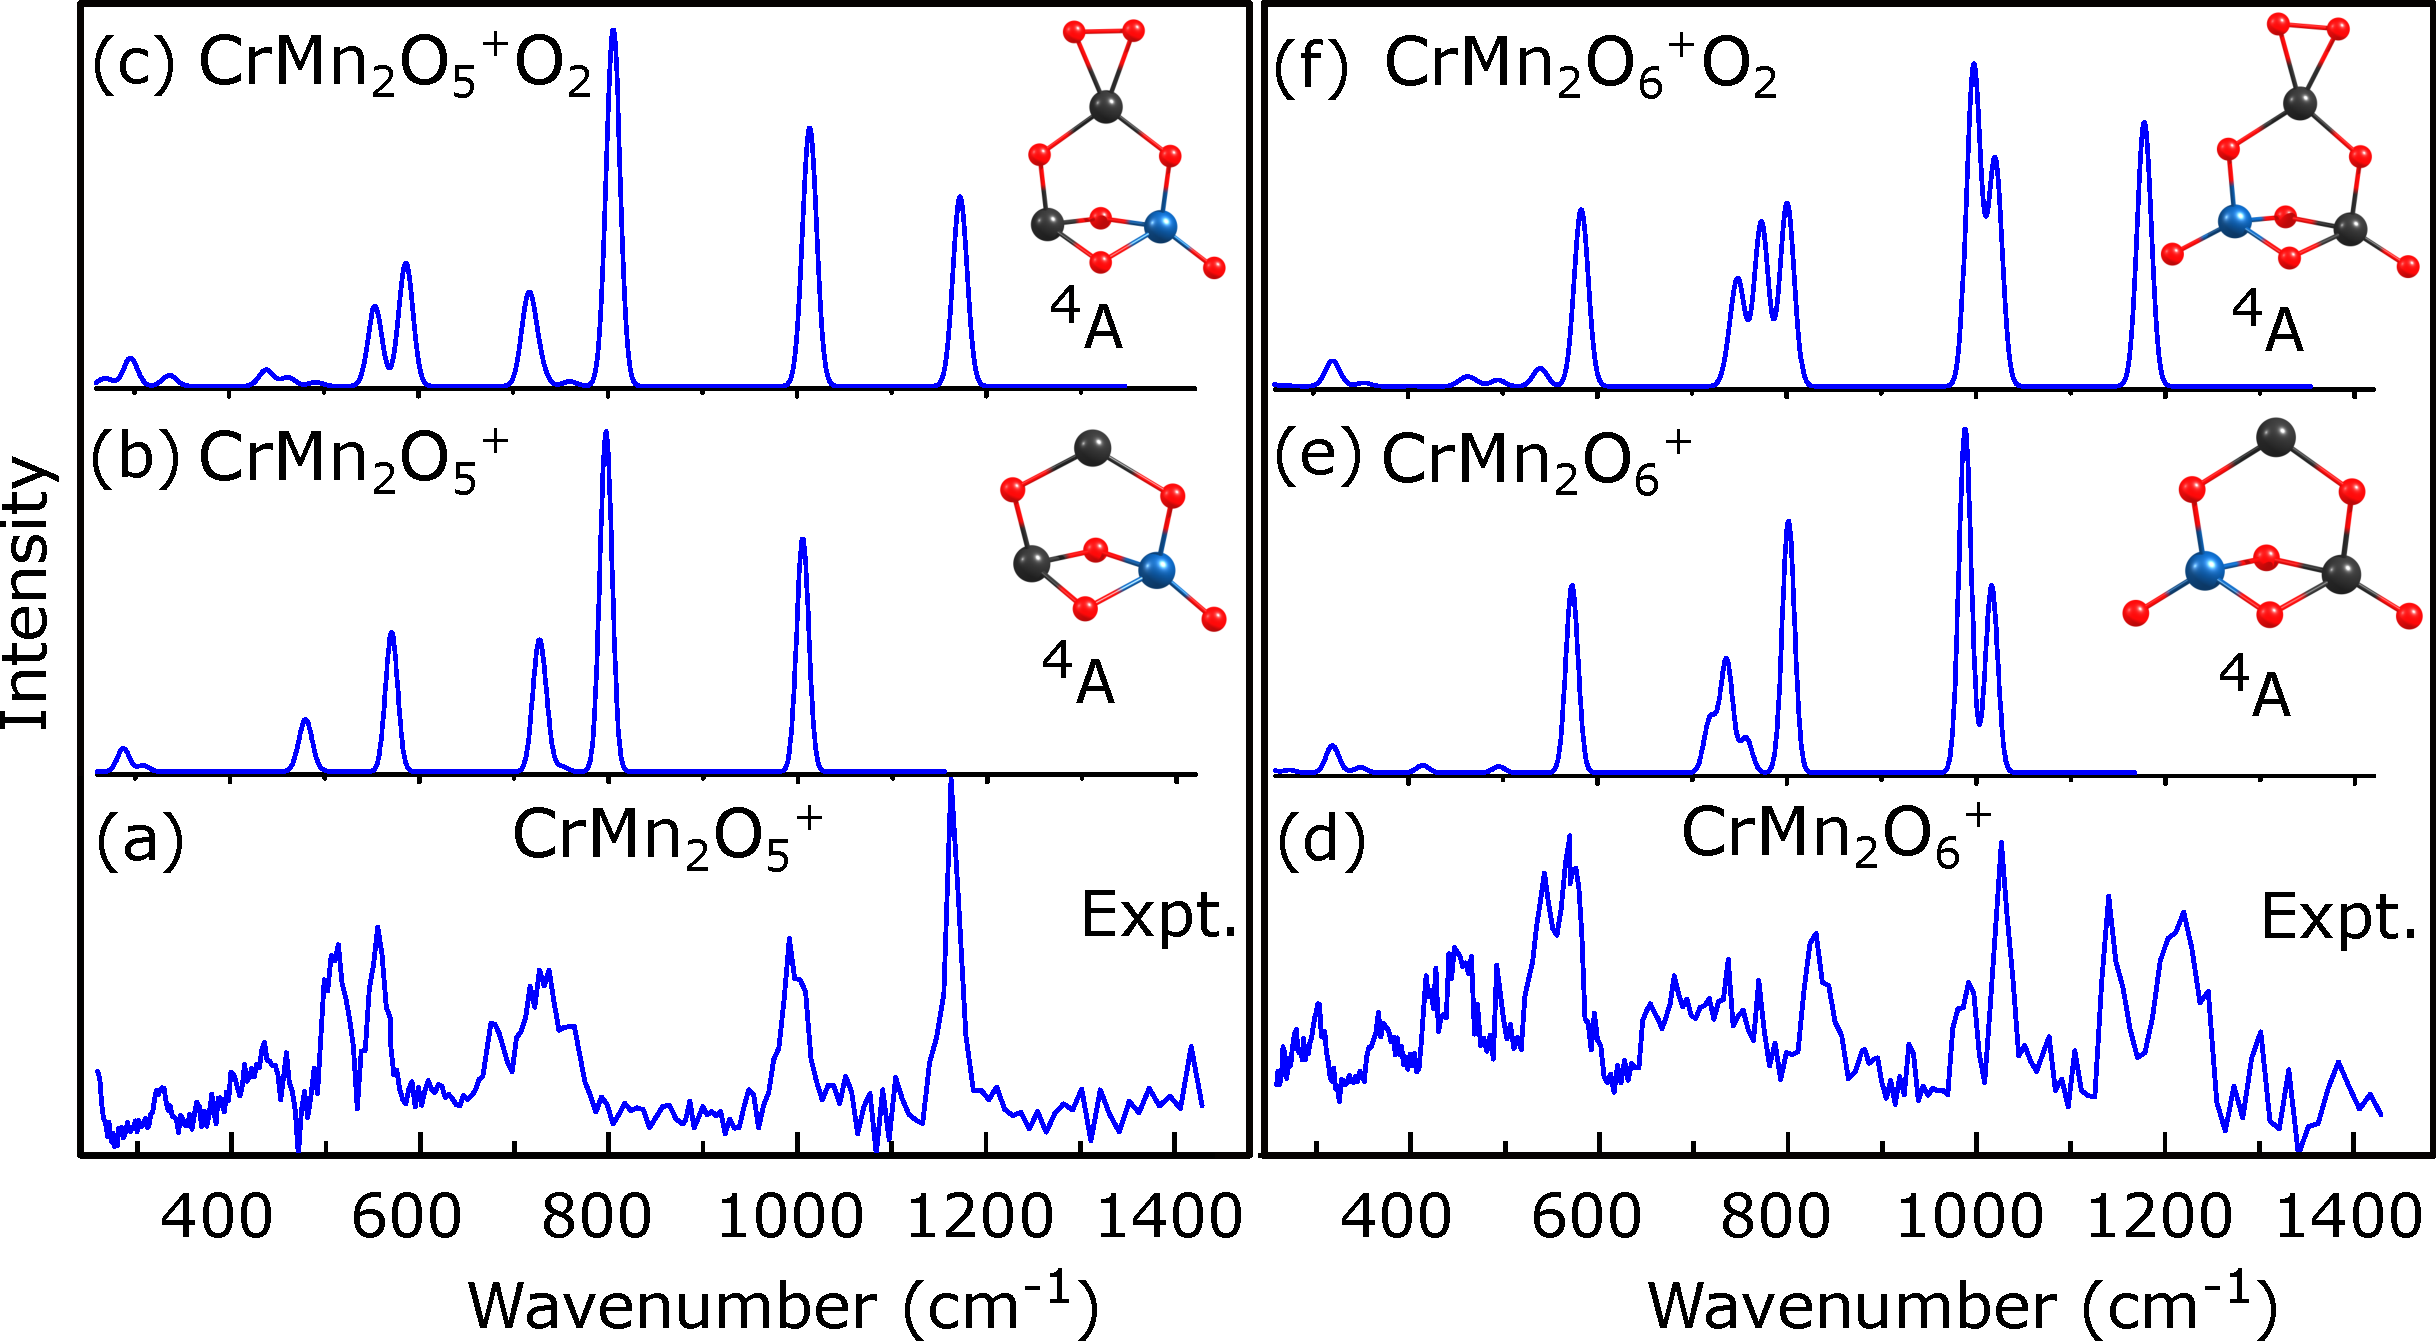
\includegraphics[width=0.8\linewidth]{CrMn2Oz}
	\caption{Experimental \acrshort{irmpd} and simulated (at the TPSS level) harmonic IR spectra of low-energy isomers of (left panel) \ch{CrMn2O5+} and (right panel) \ch{CrMn2O6+}. The geometrical structures of selected low-lying states are given as insets with chromium (manganese) atoms represented by blue (black) balls.}
	\label{fig:CrMn2Oz}
\end{figure}

The computed most stable isomers of \ch{CrMn2O5+} and \ch{CrMn2O6+} are given in subpanels b and e of Figure \ref{fig:CrMn2Oz}, respectively. Basically, the general frames of two clusters are similar with three metallic centers alternately binding to bridging oxygen atoms. The difference here is that the \ch{CrMn2O5+} has only one terminal oxygen atom binding to a chromium atom whereas in \ch{CrMn2O6+} the terminal oxygen atoms are attached to the Cr and a Mn atom. The simulated spectra of these two clusters without effects of environmental \ch{O=O} fragments successfully reproduce the experiment in the spectral range below 1100 cm$^{-1}$. The measured vibrational modes around $\sim$1200 cm$^{-1}$, can be reproduced as well by adding the \ch{O2} messenger molecule. The simulated \ch{O=O} stretching mode of attached oxygen fragment (\ch{O2}) reflects this region quite well (see parts c and f of Figure \ref{fig:CrMn2Oz}). Note that \ch{CrMn2O5+} and \ch{CrMn2O6+} have the same spin state ($^4$A). Other nearly degenerate states and energetically close isomers of \ch{CrMn2O5+} are provided in the SI.



For \ch{Cr2MnO6+}, two spin states ($^5$A and $^7$A) of the same geometrical motif, similar to the ground state of \ch{CrMn2O6+}, found to be energetically degenerate. Simulated vibrational spectra of those states are similar and nicely agree with the experiment spectrum if the \ch{O2} messenger is included in the simulation (Figure \ref{fig:Cr2MnOz}a). Since both states are energetically degenerate and their simulated spectra are nearly identical, we predict that they are both populated in the experiment.

\begin{figure}
	\centering
	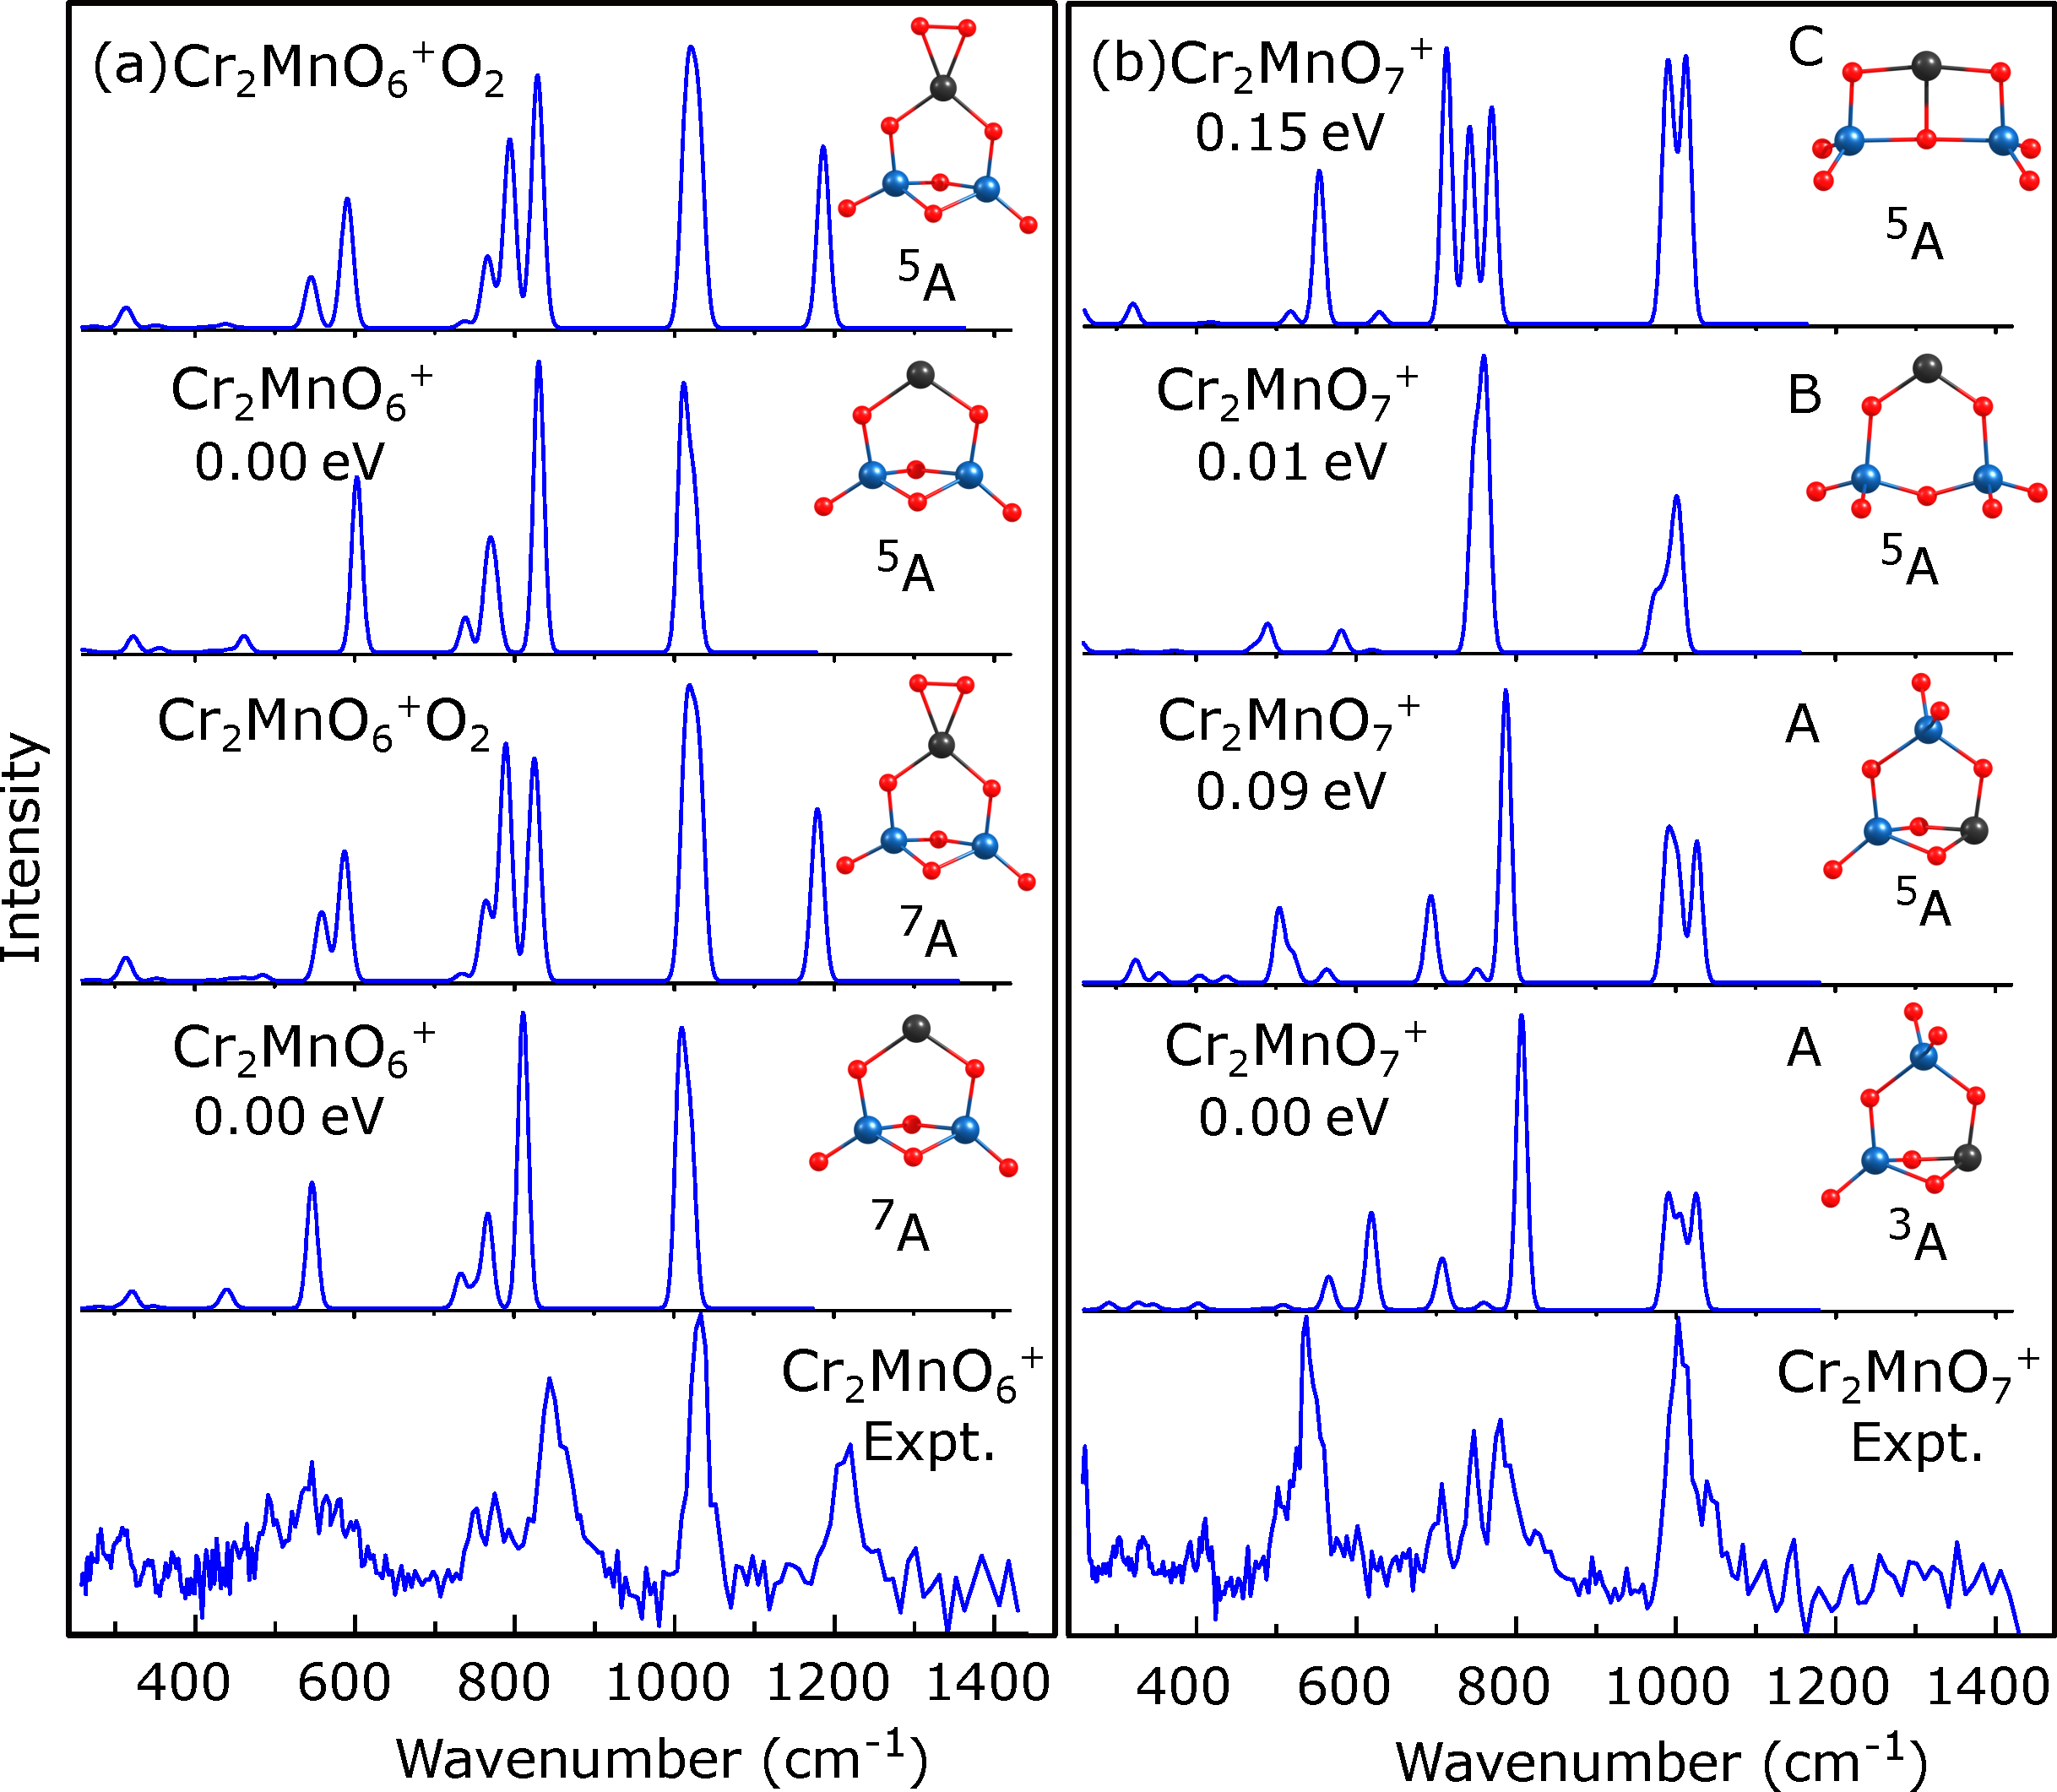
\includegraphics[width=0.8\linewidth]{Cr2MnOz}
	\caption{Experimental \acrshort{irmpd} and simulated (at the TPSS level) harmonic IR spectra of low-energy isomers of (a) \ch{Cr2MnO6+} and (b) \ch{Cr2MnO7+}. The geometrical structures of selected low-lying states are given as insets with chromium (manganese) atoms represented by blue (black) balls.}
	\label{fig:Cr2MnOz}
\end{figure}


The experimental \acrshort{irmpd} spectrum of \ch{Cr2MnO7+} does not show a band around 1200 cm$^{-1}$. This suggests that the \ch{O2} group loosely binds to \ch{Cr2MnO7+}, and the symmetric stretching mode of \ch{O=O} is IR inactive (similar to the vibration of \ch{O2} molecules). Therefore, effects of messenger is ignored in the IR simulation for this cluster. At the TPSS level, three geometrical motifs (noted as A, B, and C in Figure \ref{fig:Cr2MnOz}b) of \ch{Cr2MnO7+} were found to be energetically competitive as the most stable isomer, in which the isomer A has two nearly degenerate spin states ($^3$A and $^5$A). Energetic ordering of these isomers is not consistent among the used functionals, however the differences are small (see Table \href{https://github.com/phamlenhan/PhDDissertation/blob/master/Chapter-8SI-Nhan-thesis-CrMnO.pdf}{\textcolor{blue}{S6}}\commenttext{\ref{SI:tbl:Cr2MnO7}}). Four TPSS IR spectra of these isomers are given in the right panel of Figure \ref{fig:Cr2MnOz}. Among these four simulated spectra, two of them ($^5$A of isomers A and C) are in better agreement with the experimental one with regard to the number of active regions and vibrational frequencies. From the simulated IR spectrum of the isomer B in Figure \ref{fig:Cr2MnOz}b ($^5$A), we can see that two peaks at $\sim$ 800cm$^{-1}$ and $\sim$1050 cm$^{-1}$ can reflect the two corresponding experimental regions, but the peak at $\sim$520 cm$^{-1}$ has quite low intensity. Therefore, we believe that the $^5$A state of the isomer B does not correspond to the experiment. Note that the simulated spectrum of the $^3$A electronic state (isomer A) cannot be considered to be causing the experimental \acrshort{irmpd} spectra of \ch{Cr2MnO7+} because its simulated spectrum (Figure  \ref{fig:Cr2MnOz}b) cannot reproduce the experimental vibrational frequency of $\sim$520 cm$^{-1}$ reasonably. 




\subsubsection{\ch{Cr_xMn_yO_z+} (x + y = 4, z = 6 -- 9)}	

Five bimetallic clusters containing four metal atoms were spectroscopically investigated \ch{CrMn3O6+}, \ch{Cr2Mn2O_{7,8}+}, and \ch{Cr3MnO_{8,9}+}. The \acrshort{irmpd} spectra of these clusters seem to be different from each other with regard to the number of vibrational regions and relative intensities among each active vibrational regions; however in the experimental spectrum of each cluster, the terminal \ch{metal-O} vibration ($\sim$1000 cm$^{-1}$) and vibrations of cluster frames ($\sim$800 cm$^{-1}$) usually appear although for specific clusters they are not so clear (refer to experimental subpanels in Figures \ref{fig:CrMn3O6}, \ref{fig:Cr2Mn2Oz}, and \ref{fig:Cr3MnOz} for more details).


\begin{figure}[!htb]
	\centering
	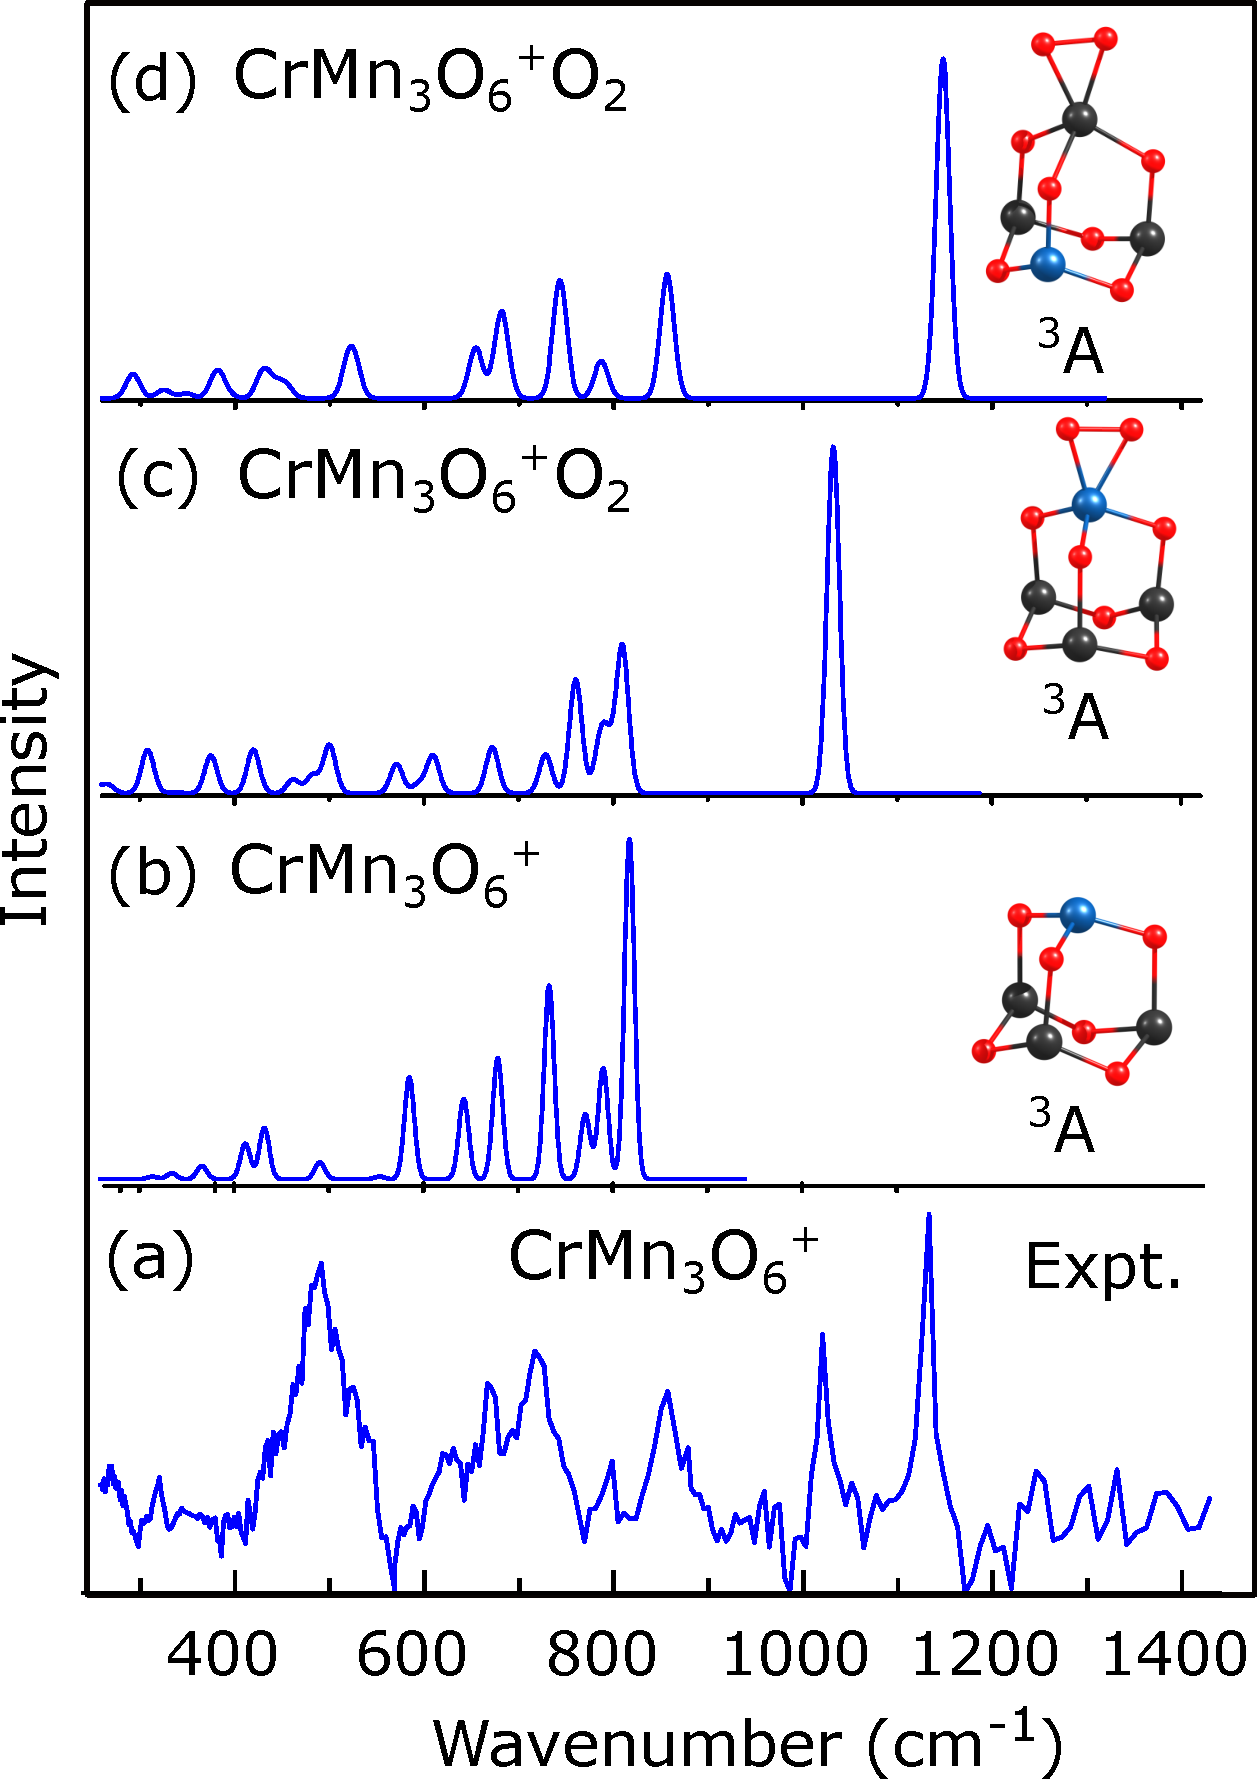
\includegraphics[width=0.4\linewidth]{CrMn3O6}
	\caption{Experimental \acrshort{irmpd} and simulated harmonic IR spectra of \ch{CrMn3O6+} at the TPSS level. The geometrical structures of selected low-lying states are given as insets with chromium (manganese) atoms represented by blue (black) balls.}
	\label{fig:CrMn3O6}
\end{figure}



The \acrshort{irmpd} spectrum of \ch{CrMn3O6+} (Figure \ref{fig:CrMn3O6}a) has five clear regions (peaks) of vibrations with high signal-to-noise ratio. Computational determination of the most stable geometrical motif and the electronic ground state of this cluster is quite challenging. Three used functionals (TPSS, B3P86, and BP86) gave three different ground-state isomers (noted as A, B, and C in Figure \href{https://github.com/phamlenhan/PhDDissertation/blob/master/Chapter-8SI-Nhan-thesis-CrMnO.pdf}{\textcolor{blue}{S7}}\commenttext{\ref{SI:figs:CrMn3O6}}), in which two isomers B and C have terminal \ch{metal-O} bonds. The isomer A (S=1) is determined as the most stable geometrical structures at the TPSS level. The predicted spectra of this isomer and its complexes with the \ch{O2} group attached to the Cr and Mn atoms are provided in subpanels b, c, and d of Figure \ref{fig:CrMn3O6}, respectively. Obviously, no single simulated spectra can reproduce two peaks at $\sim$1010 and $\sim$1120 cm$^{-1}$. Interestingly, \ch{O=O} attached to Cr and Mn atoms are computationally featured with two different wavenumbers ($\sim$1010 and $\sim$1120 cm$^{-1}$) as plotted in subpanels c and d of Figure \ref{fig:CrMn3O6}. Suppose that two complexes of \ch{CrMn3O6^+O2} were formed simultaneously and their vibrational features were observed experimentally. Two experimental peaks at $\sim$1010 and $\sim$1120 cm$^{-1}$ can be caused by two stretching vibrations of the \ch{O2} group. As a result, we believe that two complexes of \ch{CrMn3O6+} with the attached \ch{O2} at Mn and Cr sites can be populated in the experiment simultaneously to cause the complicated experimental spectrum. Note that the intensity of the vibrational region at $\sim$500 cm$^{-1}$ in the experimental spectrum is much higher than those of corresponding vibrational regions in the simulated spectra (see parts c and d of Figure \ref{fig:CrMn3O6}).


\FloatBarrier



The \acrshort{irmpd} spectrum of \ch{Cr2Mn2O7+} can be seen in Figure \ref{fig:Cr2Mn2Oz}a and is well resolved with three vibrational regions. There is no characteristic band at $\sim$1200cm$^{-1}$. Relative energies calculated using three abovementioned functionals inconsistently pointed out two structural motifs as candidates for the most stable isomer, depending on the used functionals (see the SI for relative energies). The TPSS and B3P86 functionals determined the isomer A depicted in Figure \href{https://github.com/phamlenhan/PhDDissertation/blob/master/Chapter-8SI-Nhan-thesis-CrMnO.pdf}{\textcolor{blue}{S9}}\commenttext{\ref{SI:figs:Cr2Mn2O7}} of the SI as the most stable isomer, while BP86  has a slight preference for the isomer B (see insets in parts b and c of Figure \ref{fig:Cr2Mn2Oz}). A comparison between the experimental and simulated spectra rules out the isomer A and its \ch{O2}-attached clusters (\ch{Cr2Mn2O7^+O2}) as the populated structure in the experiment because only two clear simulated peaks at $\sim$770 cm$^{-1}$ and $\sim$1005 cm$^{-1}$ are present in the simulated spectra (see Figure \href{https://github.com/phamlenhan/PhDDissertation/blob/master/Chapter-8SI-Nhan-thesis-CrMnO.pdf}{\textcolor{blue}{S44}}\commenttext{\ref{SI:figs:Cr2Mn2O7-spec-si}}). As mentioned above, no bands at $\sim$1200 cm$^{-1}$ are observed in the experimental \acrshort{irmpd} spectrum. This can be due to very weak interaction between the cluster \ch{Cr2Mn2O7+} and the \ch{O2} group, resulting in totally symmetric stretching vibrations of \ch{O=O} and then the inactive IR mode. This motivated us to focus more on the bare cluster \ch{Cr2Mn2O7+} without the effects of gas messenger. A doublet state ($^2$A) of the isomer B produces its simulated spectrum with three apparent active regions corresponding well to three pronounced experimental regions. Surprisingly, the cluster with attached \ch{O2} group (see Figure \ref{fig:Cr2Mn2Oz}d) also has three apparent active regions corresponding to three clear experimental bands but different relative intensity. The stretching vibration of the \ch{O=O} group and terminal Cr-O vibration are in the same region of $\sim$1000 cm$^{-1}$. Comparing two simulated spectra in parts c and d of Figure \ref{fig:Cr2Mn2Oz}, one can conclude that the spectrum of the bare cluster is in better agreement with the experiment. Therefore, the doublet state of the isomer B is believed to be populated in the experiment and causes the observed experimental \acrshort{irmpd} spectrum of \ch{Cr2Mn2O7+}. One other state ($^4$A) of the isomer B is $\sim$0.10 eV more stable than the $^2$A state, but its simulated IR spectrum and simulated spectra (see subpanels d and e of Figure \href{https://github.com/phamlenhan/PhDDissertation/blob/master/Chapter-8SI-Nhan-thesis-CrMnO.pdf}{\textcolor{blue}{S44}}\commenttext{\ref{SI:figs:Cr2Mn2O7-spec-si}}) of cluster-\ch{O2} are not in agreement with the experimental one; therefore this state is not populated in the experiment.  


%%% Use this for structural revolution%%% One can see that geometrical motifs of \ch{Cr2Mn2O7+} and \ch{CrMn3O7+} clusters are similar (insets in Figure \ref{fig:Cr2Mn2Oz}a versus Figure \ref{fig:CrMn3Oz}g).  


\begin{figure}[!htb]
	\centering
	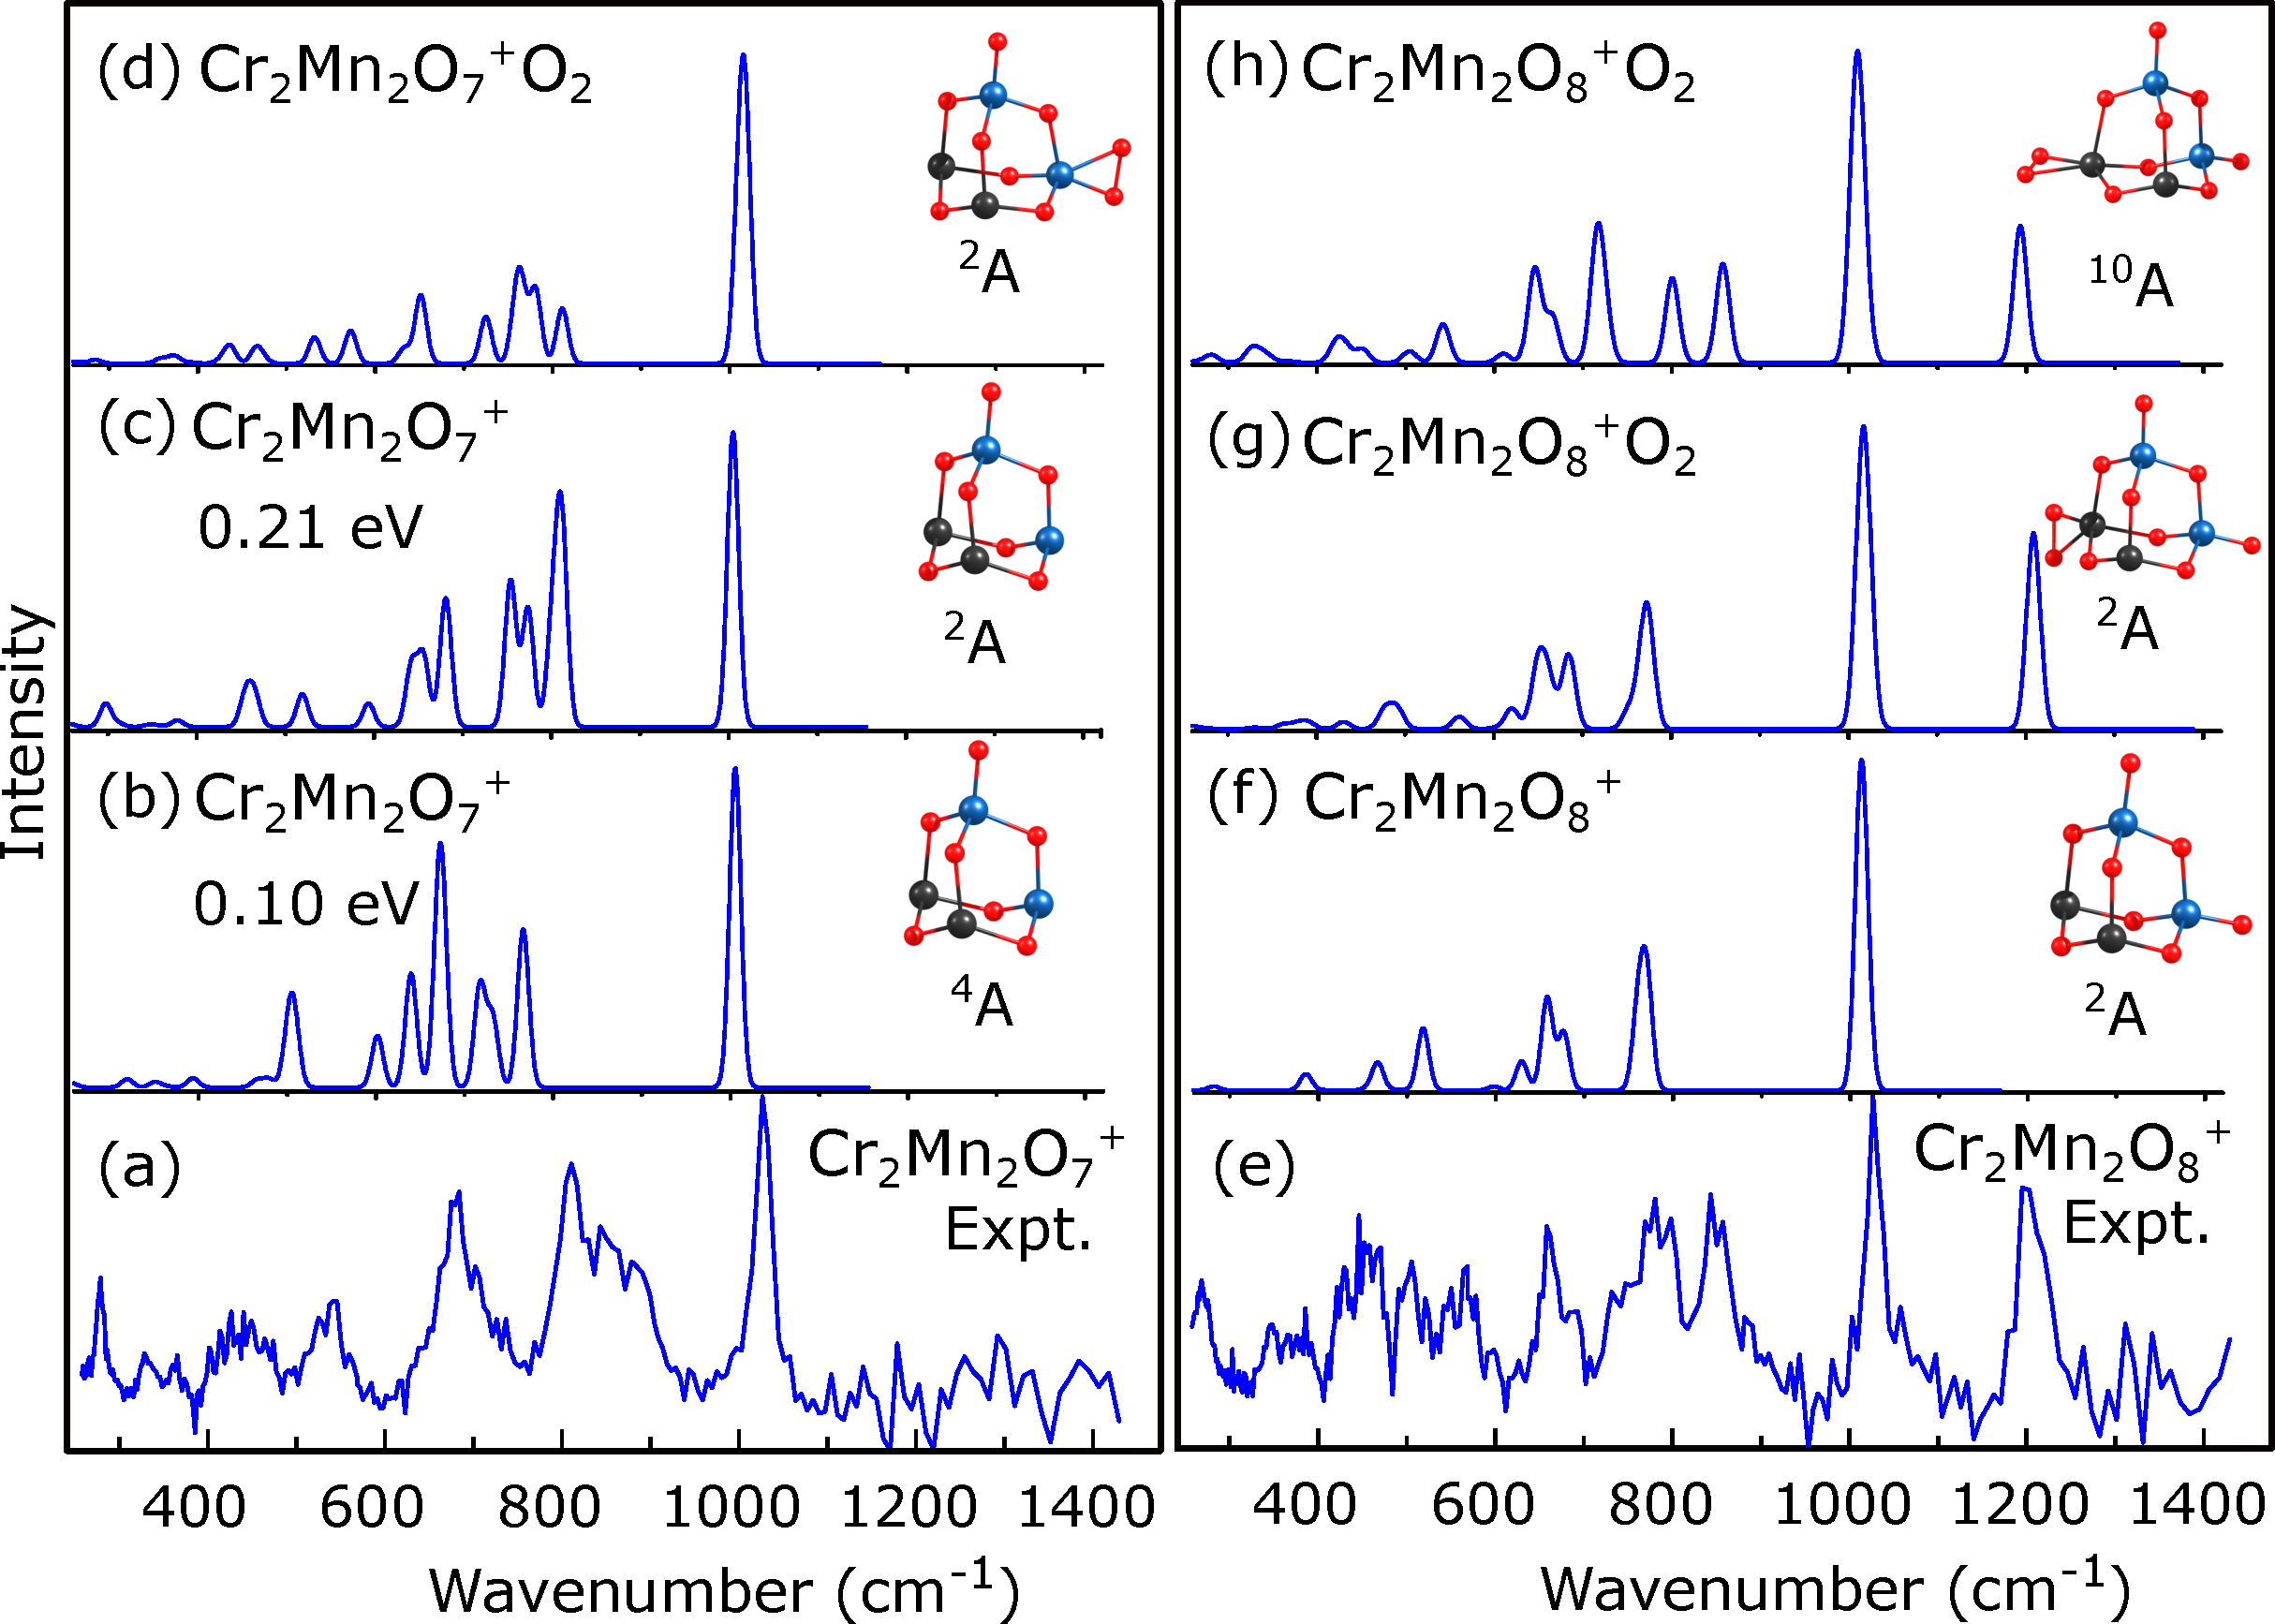
\includegraphics[width=0.8\linewidth]{Cr2Mn2Oz}
	\caption{Experimental \acrshort{irmpd} and simulated harmonic IR spectra of \ch{Cr2Mn2O_z+} (z = 7, 8) at the TPSS level. The geometrical structures of selected low-lying states are given as insets with chromium (manganese) atoms represented by blue (black) balls.}
	\label{fig:Cr2Mn2Oz}
\end{figure}






Addition of one more oxygen atom to \ch{Cr2Mn2O7+} to form \ch{Cr2Mn2O8+} does not significantly affect the main geometrical frame of clusters. Indeed, our calculations proved that the addition of one more oxygen atom creates one more terminal \ch{Cr-O} bond (second one) on the main frame of oxide clusters (inset in Figure \ref{fig:Cr2Mn2Oz}f). Such terminal \ch{Cr-O} bonds underlie harmonic vibrational frequencies of $\sim$1020 cm$^{-1}$ in the experimental \acrshort{irmpd} spectrum of \ch{Cr2Mn2O8+} (Figure \ref{fig:Cr2Mn2Oz}e). The vibrational peak at $\sim$1200 cm$^{-1}$ in the experiment is attributed to the stretching vibration of the \ch{O=O} group. IR simulation of the $^2$A ground-state structure taking account of \ch{O=O} effects reasonably reproduces two peaks at > 1000 cm$^{-1}$ in Figure \ref{fig:Cr2Mn2Oz}g. All remaining experimental peaks with frequencies of < 900 cm$^{-1}$ have rather low signal-to-noise ratio. Nevertheless, the TPSS simulated spectrum of the ground state also can reflect these features within this range. The simulated spectrum of a sextet state (the first excited state at the TPSS level) in Figure \href{https://github.com/phamlenhan/PhDDissertation/blob/master/Chapter-8SI-Nhan-thesis-CrMnO.pdf}{\textcolor{blue}{S45b}}\commenttext{\ref{SI:figs:Cr2Mn2O8-spec-si}b} has poor agreement with the experimental spectrum. Hence, it is not responsible for the experiment, although this sate was determined to be the ground state of \ch{Cr2Mn2O8+} by the BP86 functional. From experimentally populated electronic states of two clusters \ch{Cr2Mn2O7+} and \ch{Cr2Mn2O8+}, one can see that doublet spin states of these two clusters remain unchanged under variation of one oxygen atom.  



The geometrical features of \ch{Cr3MnO8+} and \ch{Cr3MnO9+} are provided in Figure \ref{fig:Cr3MnOz}. Those clusters have a similar structural motif with the additional oxygen atom in \ch{Cr3MnO9+} being attached to the third Cr atom via a terminal \ch{Cr-O} bond. From experimental spectra done for the \ch{Cr3MnO8+} and \ch{Cr3MnO9+} clusters, we can see that vibrational signals recorded are not pronounced; nonetheless, the peak at $\sim$1000 cm$^{-1}$ can still clear in both experimental spectra (Figures \ref{fig:Cr3MnOz}a and \ref{fig:Cr3MnOz}g). For \ch{Cr3MnO8+}, an unclear peak at $\sim$1200 cm$^{-1}$ seems to appear in the experimental spectrum. The same feature can be seen in the experimental spectrum of \ch{Cr3MnO9+} but at $\sim$1250 cm$^{-1}$. Since these peaks have very low intensity, it is unsure to conclude whether gas messenger really affects the experimental spectra. As a result, we consider the simulation of both with and without gas messenger. Clearly, the TPSS functional can predict the pronounced peak at $\sim$1000 cm$^{-1}$ successfully. With more attention to the experimental spectrum of \ch{Cr3MnO8+}, one recognizes all three remaining vibrational regions at < 800 cm$^{-1}$ have the quite low signal-to-noise ratio. The $^3$A ground-state of \ch{Cr3MnO8+} can reproduce all these three regions of vibrations; however one of them is $\sim$100 cm$^{-1}$ redshifted (see Figure \ref{fig:Cr3MnOz}b). The IR simulated spectrum of a distorted structure depicted in Figure \ref{fig:Cr3MnOz}e seems to have better agreement with the experiment; however the $^3$A state energy of this isomer is 1.52 eV less stable than the ground state. Taking into account of gas messenger (the \ch{O2} group), the $\sim$1200-cm$^{-1}$ peak can be reproduced but no improvements on all bands of < $\sim$1000 cm$^{-1}$ seen (see subpanels d and f in Figure \ref{fig:Cr3MnOz}). For \ch{Cr3MnO9+}, the simulated spectra of $^7$A with and without gas messenger are in better agreement with the experiment than $^5$A (see the right panel in Figure \ref{fig:Cr3MnOz}). The BP86 and B3P86 energies of these two states are nearly degenerate (see Table \href{https://github.com/phamlenhan/PhDDissertation/blob/master/Chapter-8SI-Nhan-thesis-CrMnO.pdf}{\textcolor{blue}{S12}}\commenttext{\ref{SI:tbl:Cr3MnO9}}); therefore we propose that the $^7$A state can be the ground state and it is populated in the experiment.  



\begin{figure}[!htb]
	\centering
	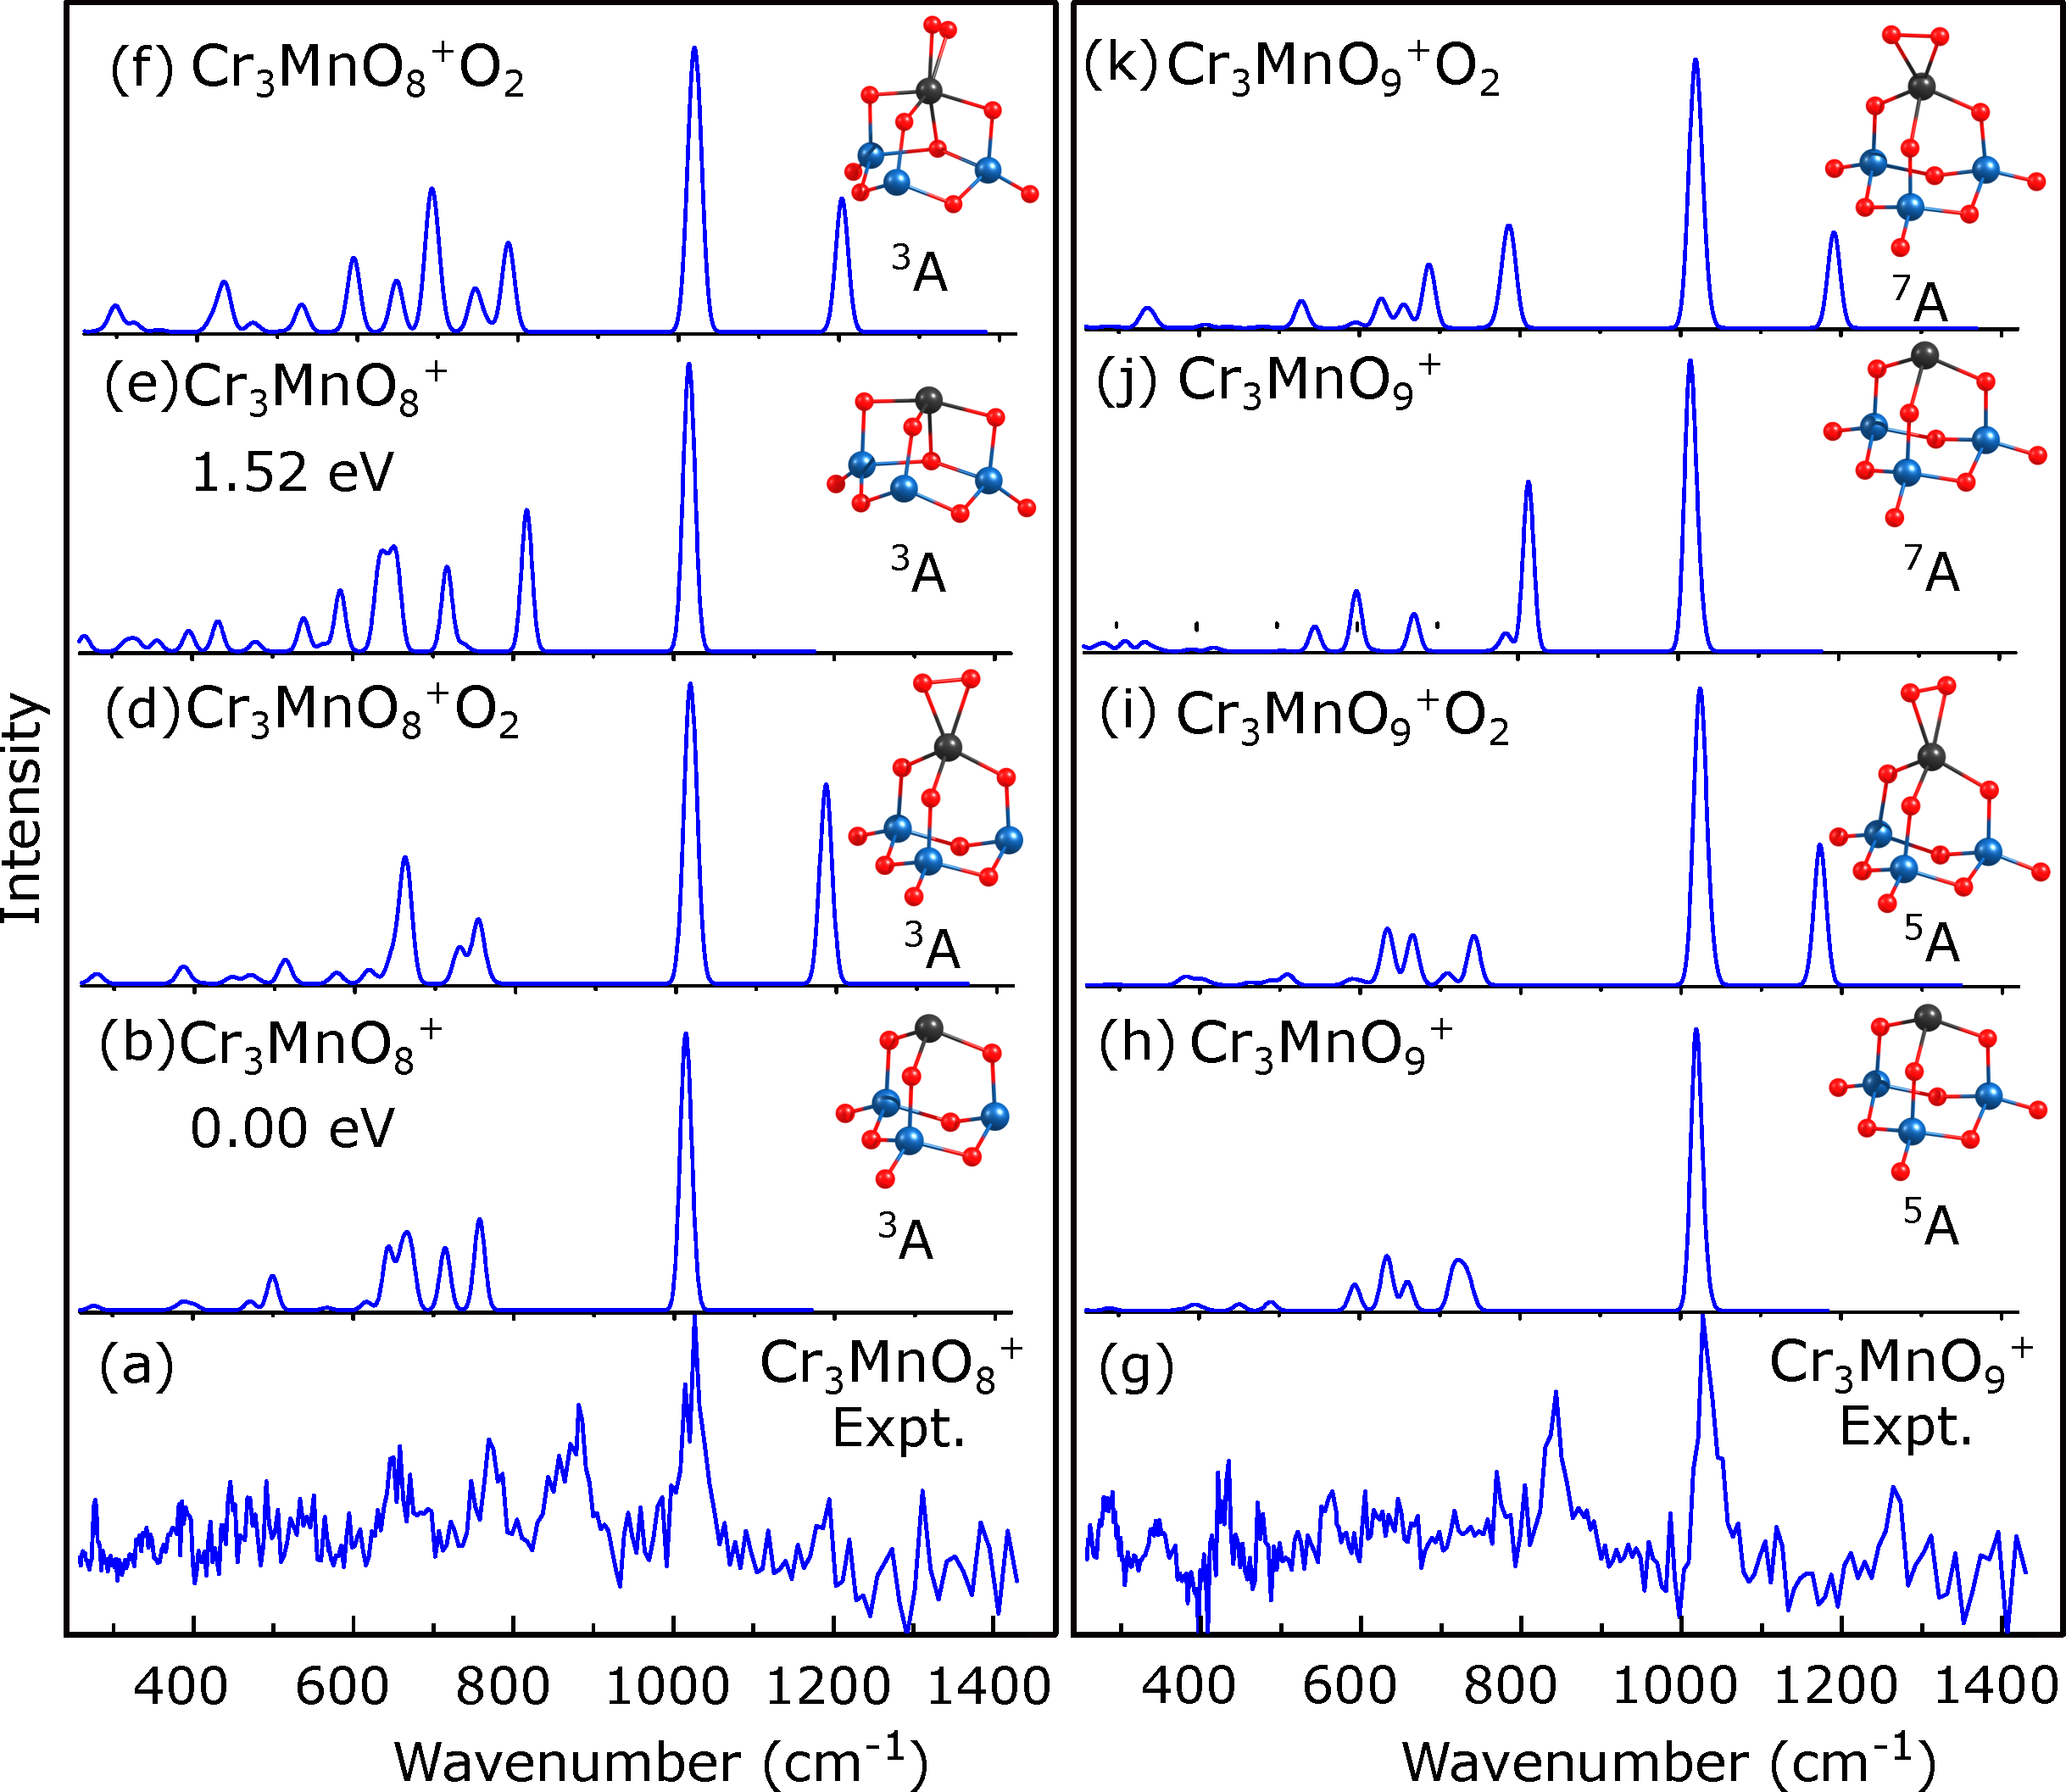
\includegraphics[width=0.8\linewidth]{Cr3MnOz}
	\caption{Experimental \acrshort{irmpd} and simulated harmonic IR spectra of \ch{Cr3MnO_z+} (z = 8, 9) at the TPSS level. The geometrical structures of selected low-lying states are given as insets with chromium (manganese) atoms represented by blue (black) balls.}
	\label{fig:Cr3MnOz}
\end{figure}


\FloatBarrier


\subsection{Structural evolution}

To explore the structural evolution of these bimetallic clusters (\ch{Cr_xMn_yO_z+}, x + y = 2 -- 4, z = 2 -- 10), several additional clusters were investigated using the TPSS functional. Geometrical structures of the predicted clusters and the above studied ones are presented in Figure \ref{fig:Struc-evo}. Below, we discuss the effects of the oxygen content, the Cr to Mn metallic ratio, and numbers of metallic atoms on the geometrical structure of the clusters.




\begin{figure}[!htb]
	\centering
	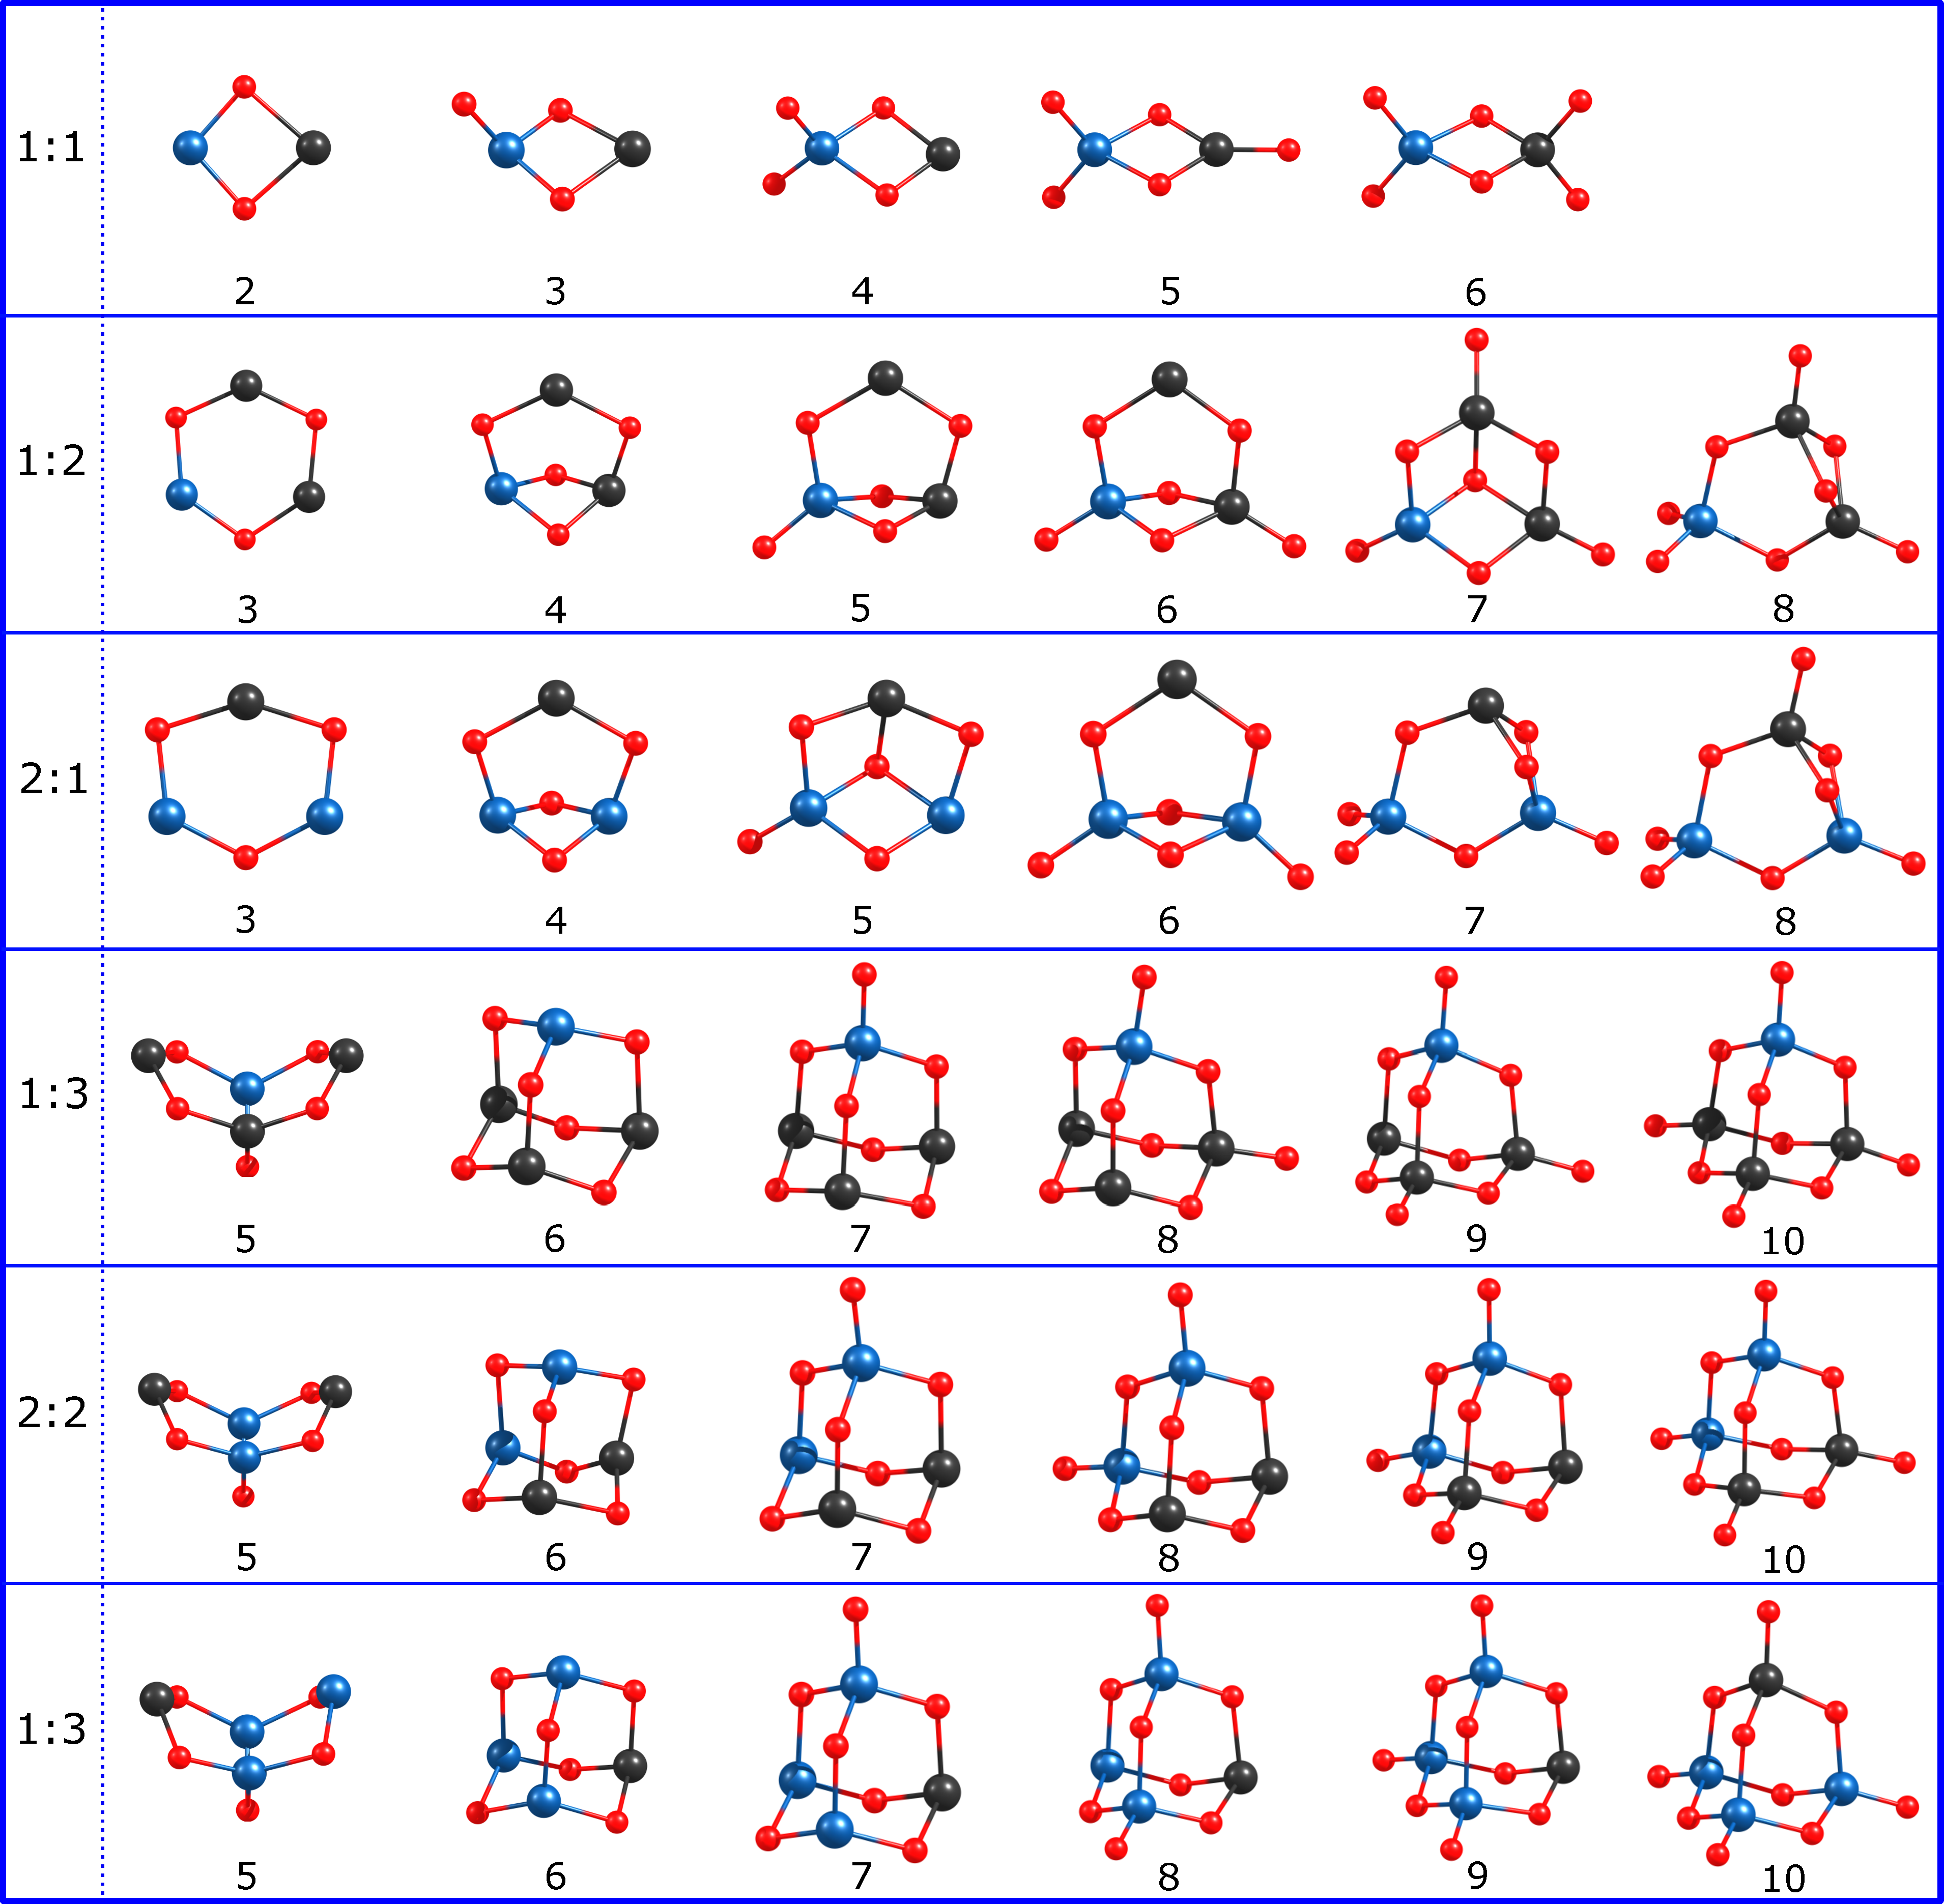
\includegraphics[width=0.8\linewidth]{Struc-evo}
	\caption{Structural evolution of \ch{Cr_xMn_yO_z+} (x + y = 2 -- 4, z = 2 -- 10). The numbers of chromium and manganese atoms are on the left-hand column, and the number of oxygen atoms is arranged horizontally below oxide structures. Chromium (manganese) balls are blue (black) balls.}
	\label{fig:Struc-evo}
\end{figure}


The metallic frame of each Cr-Mn ratio oxide series does not change under addition of oxygen atoms. Adding more oxygen atoms to clusters increases the coordination of the metallic sites. 2-fold coordination becomes 3- and 4-fold coordination when more oxygen atoms are added to a specific series of clusters. The added oxygen atoms first go to the chromium sites. Once a high oxygen coordination (3- and 4-fold) is reached for all chromium atoms, the oxygen coordination of the manganese atoms will subsequently increase under addition of more oxygen atoms. Additional oxygen atoms tend to bind first to chromium atoms and then to manganese ones. This bonding priority can be explained by the stronger \ch{Cr-O} bond in comparison to the \ch{Mn-O} one (461 $\pm$ 8.7 versus 362 $\pm$ 25 kJ mol$^{-1}$ ). \cite{Luo-2007} All oxygen atoms, except for those in terminal metal-O bonds, have 2-fold metal coordination. 


%%%The added oxygen atoms first go to the chromium sites, which prefer to have a higher oxidation state as the Mn sites.



The effects of metallic ratios can be evaluated within a specific range of oxygen atoms in \ch{Cr_xMn_yO_z+} (x + y = 3 -- 4, z = 3 -- 10). The metallic frame of series with three and four metallic atoms does not change when the metallic ratio varies. To be more specific, for the case of \ch{Cr_xMn_yO_z+} (x + y = 3) three metallic atoms are arranged to make a similar structural motif when the number of chromium atoms increases from 1 to 2. In \ch{CrMn3O_z+}, \ch{Cr2Mn2O_z+}, and \ch{Cr3MnO_z+} (z = 5 -- 10) the metallic frame is also unchanged over all possible ratios of metallic atoms.  



\subsection{Magnetic interactions}


Figure \ref{fig:Mag-mo} pictorially presents how total magnetic moments of each cluster series with two, three, and four metallic atoms varies under addition of oxygen atoms. Note that in order to see the effects of manganese on the magnetic properties, pure chromium oxide clusters with corresponding numbers of metallic atoms are also considered. For clusters with two metallic atoms, the total magnetic moment of \ch{CrMnO_z+} (z = 2 -- 6) behaves quite similarly to that of pure dichromium oxide clusters. Total magnetic moments of both series monotonically decrease under addition of oxygen atoms (see Figure \ref{fig:Mag-mo}a). In \ch{CrMnO2+}, superexchange interaction through bridging oxygen facilitates the maximum total magnetic moment as observed in \ch{Cr2O2^{-/0/+}}. \cite{Tono2003B, Nhan-Cr2O2, Nhan18} For series of clusters containing three metallic atoms,  oxygen addition does not affect total magnetic moments of \ch{CrMn2O_z+} and \ch{Cr2MnO_z+} (z = 3 -- 8) significantly (fluctuating within 2 to 5 $\mu_B$), while that of the \ch{Cr3O_z+} ( z = 3 -- 8) linearly declines from 11 to 1 $\mu_B$ because 3\textit{d} electrons of chromium are captured by additional oxygen atoms. \cite{Nhan18} Evolution of total magnetic moments in clusters with four metallic atoms is more complicated and likely dependent on the precise amount of both oxygen and chromium atoms. The addition of oxygen atoms has its stronger magnetic effects on clusters with dominant chromium ratio (3 and 4 atoms). This can be seen in Figure \ref{fig:Mag-mo}c where the total magnetic moments of these two series drastically go down from $\sim$11 to $\sim$2 $\mu_B$ when the number of oxygen atom increases from 6 to 8. In the other two series of clusters \ch{Cr2Mn2O_z+} and \ch{CrMn3O_z+} (z = 6 -- 8), the total magnetic moment fluctuates around 2 $\mu_B$. Through the evolution of total magnetic moments, we can see that introduction of manganese into oxide clusters keeps total magnetic moments lower and more stable under addition of oxygen atoms with respect to corresponding pure chromium oxide clusters. This kind of magnetic effects can be obviously observed in the series with three metallic atoms (\ch{CrMn2O_z+} and \ch{Cr2MnO_z+}). In the series with four metallic atoms, manganese playing as magnetic reducer and stabilizer can be seen in clusters with significant ratio of manganese atoms such as \ch{Cr2Mn2O_z+} and \ch{CrMn3O_z+}. To see more details about the magnetic-reducer role of manganese in the manganese-rich clusters, total magnetic moments of four clusters (\ch{Cr4O6+}, \ch{Cr3MnO6+}, \ch{Cr2Mn2O6+}, and \ch{CrMn3O6+}) and the local magnetic orientation of metallic sites within each cluster are provided in Figure \ref{fig:moment}. Apparently, the total magnetic moment plunges from around 9 to 2 $\mu_B$ when the number of manganese atoms becomes dominant in the clusters. In \ch{Cr2Mn2O6+} and \ch{CrMn3O6+}, antiferromagnetic coupling between two metallic sites appear resulting in reduction of total magnetic moments in these two clusters. Besides, moduli of local magnetic moments on the Cr sites, which are the main magnetic components causing high total magnetic moments in \ch{Cr4O6+} and \ch{Cr3MnO6+}, are also significantly reduced (see Table \href{https://github.com/phamlenhan/PhDDissertation/blob/master/Chapter-8SI-Nhan-thesis-CrMnO.pdf}{\textcolor{blue}{S43}}\commenttext{\ref{SI:tab:localmaget}}). 


\begin{figure}[!htb]
	\centering
	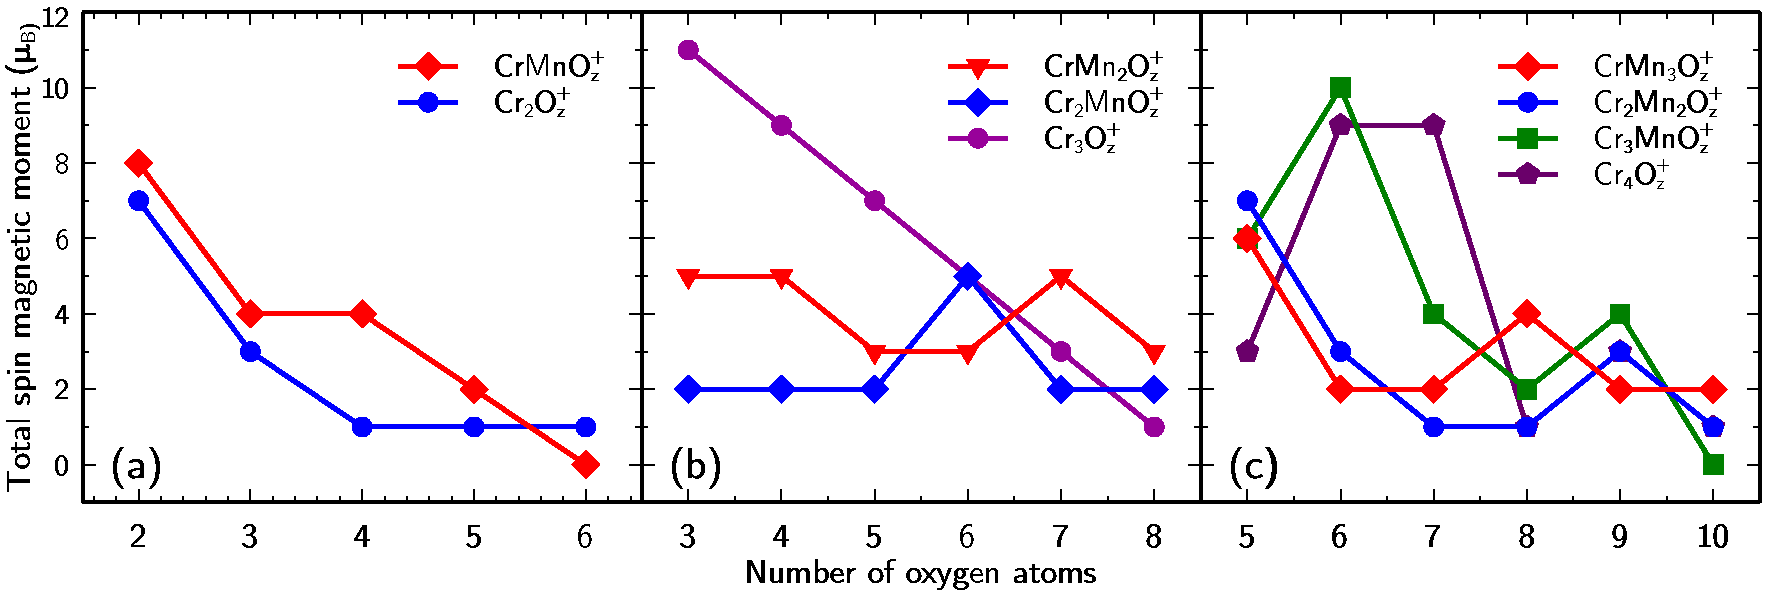
\includegraphics[width=\linewidth]{Mag-mo}
	\caption{Total magnetic moments of \ch{Cr_xMn_yO_z+} (x + y = 2 – 4, z = 2 – 10)}
	\label{fig:Mag-mo}
\end{figure}

\begin{figure}[!htb]
	\centering
	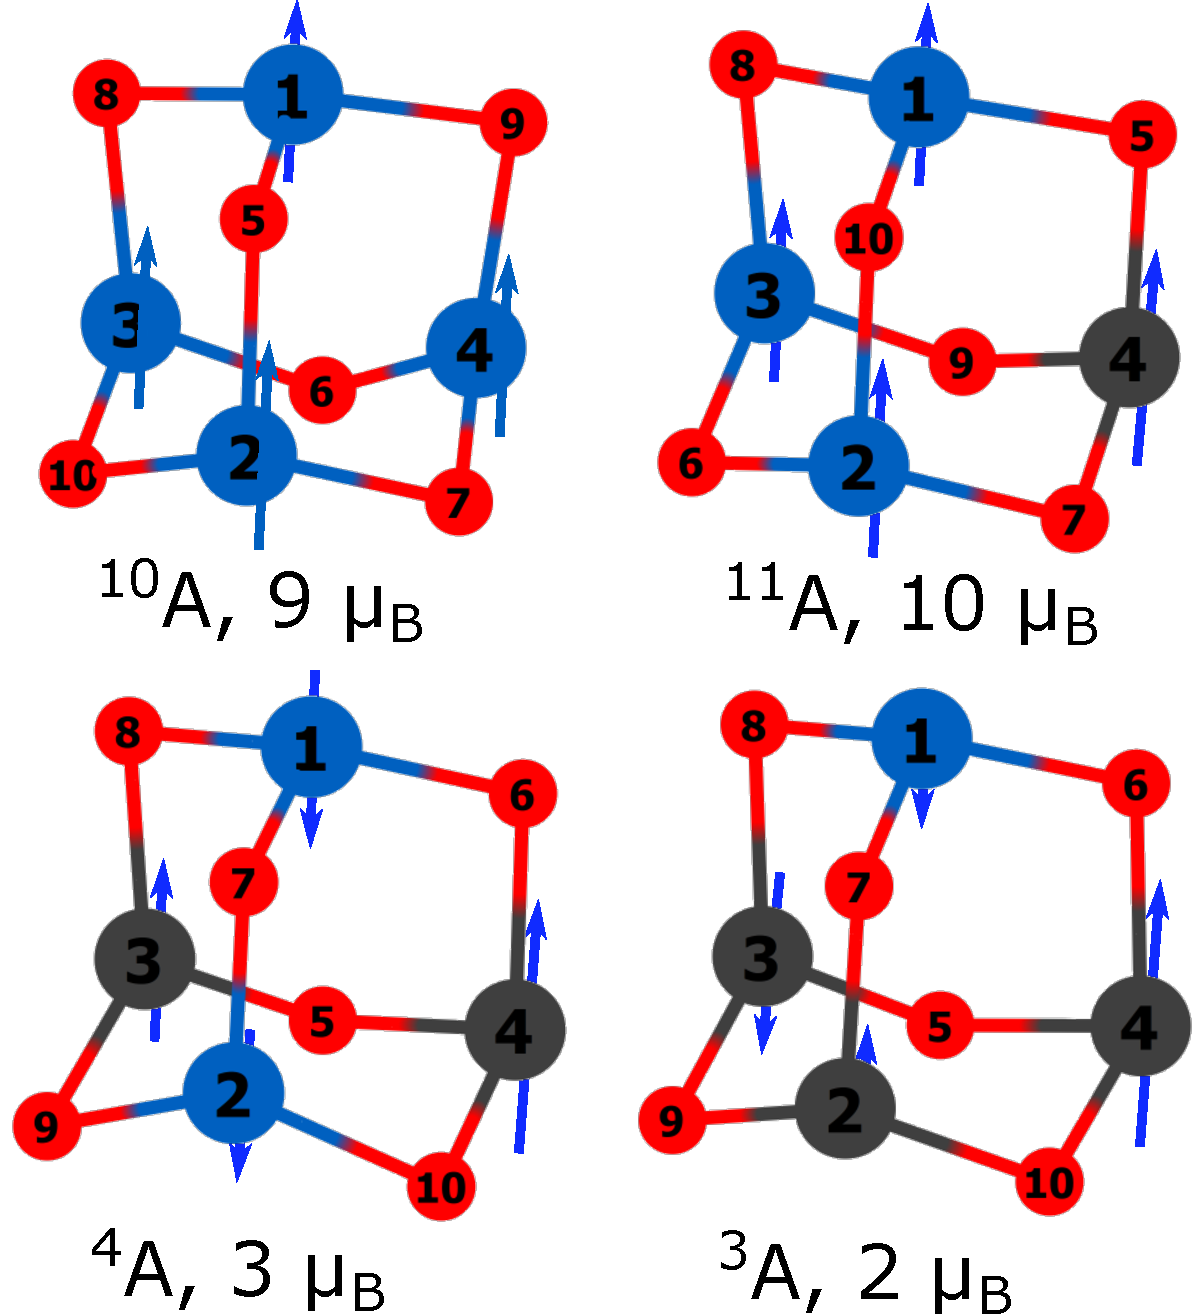
\includegraphics[width=0.4\linewidth]{magnetic-moment.pdf}
	\caption{Total magnetic moments and the orientation of the local spin magnetic moments on the metallic sites (chromium and manganese) withdrawn from natural bond orbital (NBO) analysis using the TPSS electron density. Chromium (manganese) atoms are represented by blue (black) balls.}
	\label{fig:moment}
\end{figure}

\FloatBarrier

To see how local magnetic moments of manganese and chromium sites contribute to total magnetic moments and are affected upon the addition of oxygen atoms, averaged absolute local magnetic moments (ALMMs) of each metallic element (chromium and manganese) are calculated and graphically given in Figure \ref{fig:Ave-mo}. Apparently, ALMMs of both chromium and manganese are inversely proportional to the number of oxygen atoms. Local magnetic moments of metallic sites are quenched when the number of oxygen atoms is large enough (6, 8, and 10 for clusters containing 2, 3, and 4 metallic atoms, respectively). In most of the bimetallic clusters, ALMMs of manganese are higher than those of chromium, and ALMMs of chromium in the pure chromium oxide clusters are in between those of manganese and chromium in the bimetallic ones. This local magnetic ordering suggests that electron transfer from chromium atoms to manganese ones significantly controls total magnetic moments of hybrid Cr-Mn oxide clusters, and in these hybrid oxide clusters manganese sites predominantly cause magnetic behaviors. This result can be seen intuitively for the case of four metallic clusters \ch{Cr4O6+}, \ch{Cr3MnO6+}, \ch{Cr2Mn2O6+}, and \ch{CrMn3O6+} in Figure \ref{fig:moment}.

\begin{figure}[!htb]
	\centering
	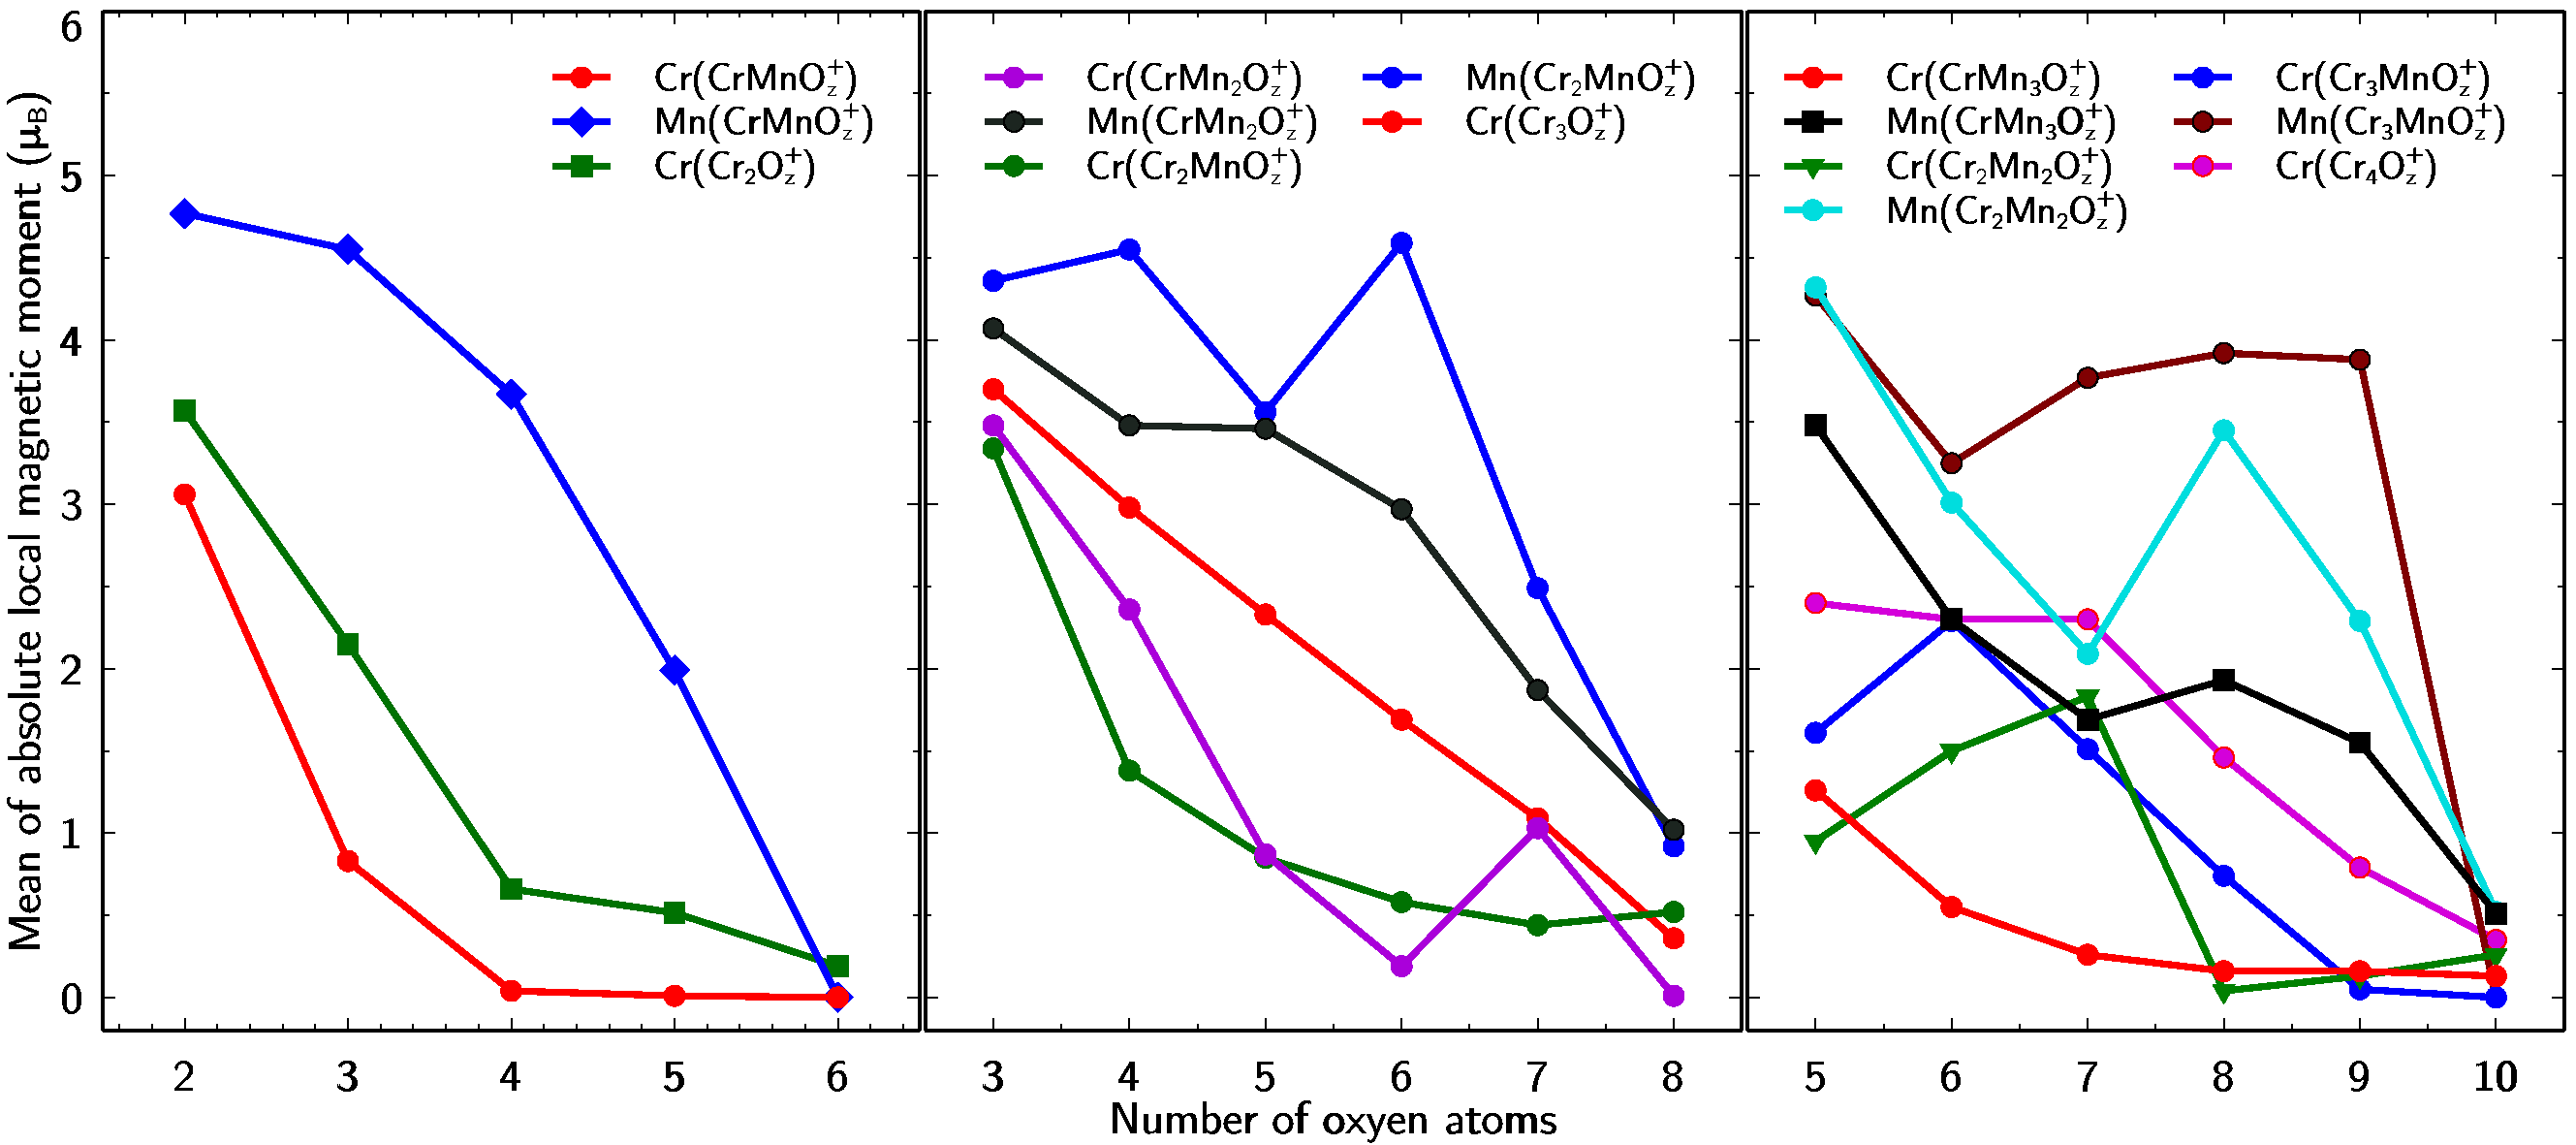
\includegraphics[width=\linewidth]{Ave-mag.pdf}
	\caption{Averaged absolute local magnetic moments of Cr and Mn in \ch{Cr_xMn_yO_z+} (x + y = 2 -- 4, z = 2 -- 10). All values were calculated from natural bond orbital (NBO) analysis using the TPSS electron density.}
	\label{fig:Ave-mo}
\end{figure}





	
%!TODO: + Is it possible that electron transfer from Chromium to manganese reduces total magnetic moments.
	
%!TODO: - Effects of metal ratio on the magnetic properties 


\subsection{Conclusion}


Various hybrid Cr-Mn oxide clusters were synthesized and characterized with the \acrshort{irmpd} technique. In combination with DFT calculations, all experimentally synthesized clusters with 2 to 4 metallic atoms were geometrically and electronically identified. Within studied clusters, general geometric frames of all series are not affected by additional oxygen atoms and metallic ratios. Several clusters possess nearly degenerate electronic states which are simultaneously populated and contribute to their experimental \acrshort{irmpd} spectra. Under addition of oxygen atoms, chromium sites tend to attract additional oxygen atoms first to reach 3- and 4-fold coordination and then to manganese sites. 


While total magnetic moments of pure chromium oxide \ch{Cr_xO_y+} and small hybrid oxide \ch{CrMnO_z+} clusters strongly depend on amount of oxygen atoms, those of bigger bimetallic ones are more stable and smaller. In these hybrid clusters, manganese plays as magnetic stabilizer and reducer. Averaged absolute local magnetic moments of manganese are much higher than those of chromium in all bimetallic clusters and higher than those of chromium in corresponding pure chromium oxide clusters. This points out that electron transfer from chromium to manganese happens. This electron transfer process and electrons captured by oxygen atoms control magnetic behaviors of bimetallic Cr-Mn oxide clusters.   






%%%%%%%%%%%%%%%%%%%%%%%%%%%%%%%%%%%%%%%%%%%%%%%%%%
% Keep the following \cleardoublepage at the end of this file, 
% otherwise \includeonly includes empty pages.
%\cleardoublepage





\includebibliography
\printbibliography[heading=subbibliography] % print section bibliography



\end{refsection}